\documentclass[10pt]{article} % For LaTeX2e
\usepackage[preprint]{tmlr}
% If accepted, instead use the following line for the camera-ready submission:
%\usepackage[accepted]{tmlr}
% To de-anonymize and remove mentions to TMLR (for example for posting to preprint servers), instead use the following:
%\usepackage[preprint]{tmlr}

% Optional math commands from https://github.com/goodfeli/dlbook_notation.
%%%%% NEW MATH DEFINITIONS %%%%%

\usepackage{amsmath,amsfonts,bm}

% Mark sections of captions for referring to divisions of figures
\newcommand{\figleft}{{\em (Left)}}
\newcommand{\figcenter}{{\em (Center)}}
\newcommand{\figright}{{\em (Right)}}
\newcommand{\figtop}{{\em (Top)}}
\newcommand{\figbottom}{{\em (Bottom)}}
\newcommand{\captiona}{{\em (a)}}
\newcommand{\captionb}{{\em (b)}}
\newcommand{\captionc}{{\em (c)}}
\newcommand{\captiond}{{\em (d)}}

% Highlight a newly defined term
\newcommand{\newterm}[1]{{\bf #1}}


% Figure reference, lower-case.
\def\figref#1{figure~\ref{#1}}
% Figure reference, capital. For start of sentence
\def\Figref#1{Figure~\ref{#1}}
\def\twofigref#1#2{figures \ref{#1} and \ref{#2}}
\def\quadfigref#1#2#3#4{figures \ref{#1}, \ref{#2}, \ref{#3} and \ref{#4}}
% Section reference, lower-case.
\def\secref#1{section~\ref{#1}}
% Section reference, capital.
\def\Secref#1{Section~\ref{#1}}
% Reference to two sections.
\def\twosecrefs#1#2{sections \ref{#1} and \ref{#2}}
% Reference to three sections.
\def\secrefs#1#2#3{sections \ref{#1}, \ref{#2} and \ref{#3}}
% Reference to an equation, lower-case.
\def\eqref#1{equation~\ref{#1}}
% Reference to an equation, upper case
\def\Eqref#1{Equation~\ref{#1}}
% A raw reference to an equation---avoid using if possible
\def\plaineqref#1{\ref{#1}}
% Reference to a chapter, lower-case.
\def\chapref#1{chapter~\ref{#1}}
% Reference to an equation, upper case.
\def\Chapref#1{Chapter~\ref{#1}}
% Reference to a range of chapters
\def\rangechapref#1#2{chapters\ref{#1}--\ref{#2}}
% Reference to an algorithm, lower-case.
\def\algref#1{algorithm~\ref{#1}}
% Reference to an algorithm, upper case.
\def\Algref#1{Algorithm~\ref{#1}}
\def\twoalgref#1#2{algorithms \ref{#1} and \ref{#2}}
\def\Twoalgref#1#2{Algorithms \ref{#1} and \ref{#2}}
% Reference to a part, lower case
\def\partref#1{part~\ref{#1}}
% Reference to a part, upper case
\def\Partref#1{Part~\ref{#1}}
\def\twopartref#1#2{parts \ref{#1} and \ref{#2}}

\def\ceil#1{\lceil #1 \rceil}
\def\floor#1{\lfloor #1 \rfloor}
\def\1{\bm{1}}
\newcommand{\train}{\mathcal{D}}
\newcommand{\valid}{\mathcal{D_{\mathrm{valid}}}}
\newcommand{\test}{\mathcal{D_{\mathrm{test}}}}

\def\eps{{\epsilon}}


% Random variables
\def\reta{{\textnormal{$\eta$}}}
\def\ra{{\textnormal{a}}}
\def\rb{{\textnormal{b}}}
\def\rc{{\textnormal{c}}}
\def\rd{{\textnormal{d}}}
\def\re{{\textnormal{e}}}
\def\rf{{\textnormal{f}}}
\def\rg{{\textnormal{g}}}
\def\rh{{\textnormal{h}}}
\def\ri{{\textnormal{i}}}
\def\rj{{\textnormal{j}}}
\def\rk{{\textnormal{k}}}
\def\rl{{\textnormal{l}}}
% rm is already a command, just don't name any random variables m
\def\rn{{\textnormal{n}}}
\def\ro{{\textnormal{o}}}
\def\rp{{\textnormal{p}}}
\def\rq{{\textnormal{q}}}
\def\rr{{\textnormal{r}}}
\def\rs{{\textnormal{s}}}
\def\rt{{\textnormal{t}}}
\def\ru{{\textnormal{u}}}
\def\rv{{\textnormal{v}}}
\def\rw{{\textnormal{w}}}
\def\rx{{\textnormal{x}}}
\def\ry{{\textnormal{y}}}
\def\rz{{\textnormal{z}}}

% Random vectors
\def\rvepsilon{{\mathbf{\epsilon}}}
\def\rvtheta{{\mathbf{\theta}}}
\def\rva{{\mathbf{a}}}
\def\rvb{{\mathbf{b}}}
\def\rvc{{\mathbf{c}}}
\def\rvd{{\mathbf{d}}}
\def\rve{{\mathbf{e}}}
\def\rvf{{\mathbf{f}}}
\def\rvg{{\mathbf{g}}}
\def\rvh{{\mathbf{h}}}
\def\rvu{{\mathbf{i}}}
\def\rvj{{\mathbf{j}}}
\def\rvk{{\mathbf{k}}}
\def\rvl{{\mathbf{l}}}
\def\rvm{{\mathbf{m}}}
\def\rvn{{\mathbf{n}}}
\def\rvo{{\mathbf{o}}}
\def\rvp{{\mathbf{p}}}
\def\rvq{{\mathbf{q}}}
\def\rvr{{\mathbf{r}}}
\def\rvs{{\mathbf{s}}}
\def\rvt{{\mathbf{t}}}
\def\rvu{{\mathbf{u}}}
\def\rvv{{\mathbf{v}}}
\def\rvw{{\mathbf{w}}}
\def\rvx{{\mathbf{x}}}
\def\rvy{{\mathbf{y}}}
\def\rvz{{\mathbf{z}}}

% Elements of random vectors
\def\erva{{\textnormal{a}}}
\def\ervb{{\textnormal{b}}}
\def\ervc{{\textnormal{c}}}
\def\ervd{{\textnormal{d}}}
\def\erve{{\textnormal{e}}}
\def\ervf{{\textnormal{f}}}
\def\ervg{{\textnormal{g}}}
\def\ervh{{\textnormal{h}}}
\def\ervi{{\textnormal{i}}}
\def\ervj{{\textnormal{j}}}
\def\ervk{{\textnormal{k}}}
\def\ervl{{\textnormal{l}}}
\def\ervm{{\textnormal{m}}}
\def\ervn{{\textnormal{n}}}
\def\ervo{{\textnormal{o}}}
\def\ervp{{\textnormal{p}}}
\def\ervq{{\textnormal{q}}}
\def\ervr{{\textnormal{r}}}
\def\ervs{{\textnormal{s}}}
\def\ervt{{\textnormal{t}}}
\def\ervu{{\textnormal{u}}}
\def\ervv{{\textnormal{v}}}
\def\ervw{{\textnormal{w}}}
\def\ervx{{\textnormal{x}}}
\def\ervy{{\textnormal{y}}}
\def\ervz{{\textnormal{z}}}

% Random matrices
\def\rmA{{\mathbf{A}}}
\def\rmB{{\mathbf{B}}}
\def\rmC{{\mathbf{C}}}
\def\rmD{{\mathbf{D}}}
\def\rmE{{\mathbf{E}}}
\def\rmF{{\mathbf{F}}}
\def\rmG{{\mathbf{G}}}
\def\rmH{{\mathbf{H}}}
\def\rmI{{\mathbf{I}}}
\def\rmJ{{\mathbf{J}}}
\def\rmK{{\mathbf{K}}}
\def\rmL{{\mathbf{L}}}
\def\rmM{{\mathbf{M}}}
\def\rmN{{\mathbf{N}}}
\def\rmO{{\mathbf{O}}}
\def\rmP{{\mathbf{P}}}
\def\rmQ{{\mathbf{Q}}}
\def\rmR{{\mathbf{R}}}
\def\rmS{{\mathbf{S}}}
\def\rmT{{\mathbf{T}}}
\def\rmU{{\mathbf{U}}}
\def\rmV{{\mathbf{V}}}
\def\rmW{{\mathbf{W}}}
\def\rmX{{\mathbf{X}}}
\def\rmY{{\mathbf{Y}}}
\def\rmZ{{\mathbf{Z}}}

% Elements of random matrices
\def\ermA{{\textnormal{A}}}
\def\ermB{{\textnormal{B}}}
\def\ermC{{\textnormal{C}}}
\def\ermD{{\textnormal{D}}}
\def\ermE{{\textnormal{E}}}
\def\ermF{{\textnormal{F}}}
\def\ermG{{\textnormal{G}}}
\def\ermH{{\textnormal{H}}}
\def\ermI{{\textnormal{I}}}
\def\ermJ{{\textnormal{J}}}
\def\ermK{{\textnormal{K}}}
\def\ermL{{\textnormal{L}}}
\def\ermM{{\textnormal{M}}}
\def\ermN{{\textnormal{N}}}
\def\ermO{{\textnormal{O}}}
\def\ermP{{\textnormal{P}}}
\def\ermQ{{\textnormal{Q}}}
\def\ermR{{\textnormal{R}}}
\def\ermS{{\textnormal{S}}}
\def\ermT{{\textnormal{T}}}
\def\ermU{{\textnormal{U}}}
\def\ermV{{\textnormal{V}}}
\def\ermW{{\textnormal{W}}}
\def\ermX{{\textnormal{X}}}
\def\ermY{{\textnormal{Y}}}
\def\ermZ{{\textnormal{Z}}}

% Vectors
\def\vzero{{\bm{0}}}
\def\vone{{\bm{1}}}
\def\vmu{{\bm{\mu}}}
\def\vtheta{{\bm{\theta}}}
\def\va{{\bm{a}}}
\def\vb{{\bm{b}}}
\def\vc{{\bm{c}}}
\def\vd{{\bm{d}}}
\def\ve{{\bm{e}}}
\def\vf{{\bm{f}}}
\def\vg{{\bm{g}}}
\def\vh{{\bm{h}}}
\def\vi{{\bm{i}}}
\def\vj{{\bm{j}}}
\def\vk{{\bm{k}}}
\def\vl{{\bm{l}}}
\def\vm{{\bm{m}}}
\def\vn{{\bm{n}}}
\def\vo{{\bm{o}}}
\def\vp{{\bm{p}}}
\def\vq{{\bm{q}}}
\def\vr{{\bm{r}}}
\def\vs{{\bm{s}}}
\def\vt{{\bm{t}}}
\def\vu{{\bm{u}}}
\def\vv{{\bm{v}}}
\def\vw{{\bm{w}}}
\def\vx{{\bm{x}}}
\def\vy{{\bm{y}}}
\def\vz{{\bm{z}}}

% Elements of vectors
\def\evalpha{{\alpha}}
\def\evbeta{{\beta}}
\def\evepsilon{{\epsilon}}
\def\evlambda{{\lambda}}
\def\evomega{{\omega}}
\def\evmu{{\mu}}
\def\evpsi{{\psi}}
\def\evsigma{{\sigma}}
\def\evtheta{{\theta}}
\def\eva{{a}}
\def\evb{{b}}
\def\evc{{c}}
\def\evd{{d}}
\def\eve{{e}}
\def\evf{{f}}
\def\evg{{g}}
\def\evh{{h}}
\def\evi{{i}}
\def\evj{{j}}
\def\evk{{k}}
\def\evl{{l}}
\def\evm{{m}}
\def\evn{{n}}
\def\evo{{o}}
\def\evp{{p}}
\def\evq{{q}}
\def\evr{{r}}
\def\evs{{s}}
\def\evt{{t}}
\def\evu{{u}}
\def\evv{{v}}
\def\evw{{w}}
\def\evx{{x}}
\def\evy{{y}}
\def\evz{{z}}

% Matrix
\def\mA{{\bm{A}}}
\def\mB{{\bm{B}}}
\def\mC{{\bm{C}}}
\def\mD{{\bm{D}}}
\def\mE{{\bm{E}}}
\def\mF{{\bm{F}}}
\def\mG{{\bm{G}}}
\def\mH{{\bm{H}}}
\def\mI{{\bm{I}}}
\def\mJ{{\bm{J}}}
\def\mK{{\bm{K}}}
\def\mL{{\bm{L}}}
\def\mM{{\bm{M}}}
\def\mN{{\bm{N}}}
\def\mO{{\bm{O}}}
\def\mP{{\bm{P}}}
\def\mQ{{\bm{Q}}}
\def\mR{{\bm{R}}}
\def\mS{{\bm{S}}}
\def\mT{{\bm{T}}}
\def\mU{{\bm{U}}}
\def\mV{{\bm{V}}}
\def\mW{{\bm{W}}}
\def\mX{{\bm{X}}}
\def\mY{{\bm{Y}}}
\def\mZ{{\bm{Z}}}
\def\mBeta{{\bm{\beta}}}
\def\mPhi{{\bm{\Phi}}}
\def\mLambda{{\bm{\Lambda}}}
\def\mSigma{{\bm{\Sigma}}}

% Tensor
\DeclareMathAlphabet{\mathsfit}{\encodingdefault}{\sfdefault}{m}{sl}
\SetMathAlphabet{\mathsfit}{bold}{\encodingdefault}{\sfdefault}{bx}{n}
\newcommand{\tens}[1]{\bm{\mathsfit{#1}}}
\def\tA{{\tens{A}}}
\def\tB{{\tens{B}}}
\def\tC{{\tens{C}}}
\def\tD{{\tens{D}}}
\def\tE{{\tens{E}}}
\def\tF{{\tens{F}}}
\def\tG{{\tens{G}}}
\def\tH{{\tens{H}}}
\def\tI{{\tens{I}}}
\def\tJ{{\tens{J}}}
\def\tK{{\tens{K}}}
\def\tL{{\tens{L}}}
\def\tM{{\tens{M}}}
\def\tN{{\tens{N}}}
\def\tO{{\tens{O}}}
\def\tP{{\tens{P}}}
\def\tQ{{\tens{Q}}}
\def\tR{{\tens{R}}}
\def\tS{{\tens{S}}}
\def\tT{{\tens{T}}}
\def\tU{{\tens{U}}}
\def\tV{{\tens{V}}}
\def\tW{{\tens{W}}}
\def\tX{{\tens{X}}}
\def\tY{{\tens{Y}}}
\def\tZ{{\tens{Z}}}


% Graph
\def\gA{{\mathcal{A}}}
\def\gB{{\mathcal{B}}}
\def\gC{{\mathcal{C}}}
\def\gD{{\mathcal{D}}}
\def\gE{{\mathcal{E}}}
\def\gF{{\mathcal{F}}}
\def\gG{{\mathcal{G}}}
\def\gH{{\mathcal{H}}}
\def\gI{{\mathcal{I}}}
\def\gJ{{\mathcal{J}}}
\def\gK{{\mathcal{K}}}
\def\gL{{\mathcal{L}}}
\def\gM{{\mathcal{M}}}
\def\gN{{\mathcal{N}}}
\def\gO{{\mathcal{O}}}
\def\gP{{\mathcal{P}}}
\def\gQ{{\mathcal{Q}}}
\def\gR{{\mathcal{R}}}
\def\gS{{\mathcal{S}}}
\def\gT{{\mathcal{T}}}
\def\gU{{\mathcal{U}}}
\def\gV{{\mathcal{V}}}
\def\gW{{\mathcal{W}}}
\def\gX{{\mathcal{X}}}
\def\gY{{\mathcal{Y}}}
\def\gZ{{\mathcal{Z}}}

% Sets
\def\sA{{\mathbb{A}}}
\def\sB{{\mathbb{B}}}
\def\sC{{\mathbb{C}}}
\def\sD{{\mathbb{D}}}
% Don't use a set called E, because this would be the same as our symbol
% for expectation.
\def\sF{{\mathbb{F}}}
\def\sG{{\mathbb{G}}}
\def\sH{{\mathbb{H}}}
\def\sI{{\mathbb{I}}}
\def\sJ{{\mathbb{J}}}
\def\sK{{\mathbb{K}}}
\def\sL{{\mathbb{L}}}
\def\sM{{\mathbb{M}}}
\def\sN{{\mathbb{N}}}
\def\sO{{\mathbb{O}}}
\def\sP{{\mathbb{P}}}
\def\sQ{{\mathbb{Q}}}
\def\sR{{\mathbb{R}}}
\def\sS{{\mathbb{S}}}
\def\sT{{\mathbb{T}}}
\def\sU{{\mathbb{U}}}
\def\sV{{\mathbb{V}}}
\def\sW{{\mathbb{W}}}
\def\sX{{\mathbb{X}}}
\def\sY{{\mathbb{Y}}}
\def\sZ{{\mathbb{Z}}}

% Entries of a matrix
\def\emLambda{{\Lambda}}
\def\emA{{A}}
\def\emB{{B}}
\def\emC{{C}}
\def\emD{{D}}
\def\emE{{E}}
\def\emF{{F}}
\def\emG{{G}}
\def\emH{{H}}
\def\emI{{I}}
\def\emJ{{J}}
\def\emK{{K}}
\def\emL{{L}}
\def\emM{{M}}
\def\emN{{N}}
\def\emO{{O}}
\def\emP{{P}}
\def\emQ{{Q}}
\def\emR{{R}}
\def\emS{{S}}
\def\emT{{T}}
\def\emU{{U}}
\def\emV{{V}}
\def\emW{{W}}
\def\emX{{X}}
\def\emY{{Y}}
\def\emZ{{Z}}
\def\emSigma{{\Sigma}}

% entries of a tensor
% Same font as tensor, without \bm wrapper
\newcommand{\etens}[1]{\mathsfit{#1}}
\def\etLambda{{\etens{\Lambda}}}
\def\etA{{\etens{A}}}
\def\etB{{\etens{B}}}
\def\etC{{\etens{C}}}
\def\etD{{\etens{D}}}
\def\etE{{\etens{E}}}
\def\etF{{\etens{F}}}
\def\etG{{\etens{G}}}
\def\etH{{\etens{H}}}
\def\etI{{\etens{I}}}
\def\etJ{{\etens{J}}}
\def\etK{{\etens{K}}}
\def\etL{{\etens{L}}}
\def\etM{{\etens{M}}}
\def\etN{{\etens{N}}}
\def\etO{{\etens{O}}}
\def\etP{{\etens{P}}}
\def\etQ{{\etens{Q}}}
\def\etR{{\etens{R}}}
\def\etS{{\etens{S}}}
\def\etT{{\etens{T}}}
\def\etU{{\etens{U}}}
\def\etV{{\etens{V}}}
\def\etW{{\etens{W}}}
\def\etX{{\etens{X}}}
\def\etY{{\etens{Y}}}
\def\etZ{{\etens{Z}}}

% The true underlying data generating distribution
\newcommand{\pdata}{p_{\rm{data}}}
% The empirical distribution defined by the training set
\newcommand{\ptrain}{\hat{p}_{\rm{data}}}
\newcommand{\Ptrain}{\hat{P}_{\rm{data}}}
% The model distribution
\newcommand{\pmodel}{p_{\rm{model}}}
\newcommand{\Pmodel}{P_{\rm{model}}}
\newcommand{\ptildemodel}{\tilde{p}_{\rm{model}}}
% Stochastic autoencoder distributions
\newcommand{\pencode}{p_{\rm{encoder}}}
\newcommand{\pdecode}{p_{\rm{decoder}}}
\newcommand{\precons}{p_{\rm{reconstruct}}}

\newcommand{\laplace}{\mathrm{Laplace}} % Laplace distribution

\newcommand{\E}{\mathbb{E}}
\newcommand{\Ls}{\mathcal{L}}
\newcommand{\R}{\mathbb{R}}
\newcommand{\emp}{\tilde{p}}
\newcommand{\lr}{\alpha}
\newcommand{\reg}{\lambda}
\newcommand{\rect}{\mathrm{rectifier}}
\newcommand{\softmax}{\mathrm{softmax}}
\newcommand{\sigmoid}{\sigma}
\newcommand{\softplus}{\zeta}
\newcommand{\KL}{D_{\mathrm{KL}}}
\newcommand{\Var}{\mathrm{Var}}
\newcommand{\standarderror}{\mathrm{SE}}
\newcommand{\Cov}{\mathrm{Cov}}
% Wolfram Mathworld says $L^2$ is for function spaces and $\ell^2$ is for vectors
% But then they seem to use $L^2$ for vectors throughout the site, and so does
% wikipedia.
\newcommand{\normlzero}{L^0}
\newcommand{\normlone}{L^1}
\newcommand{\normltwo}{L^2}
\newcommand{\normlp}{L^p}
\newcommand{\normmax}{L^\infty}

\newcommand{\parents}{Pa} % See usage in notation.tex. Chosen to match Daphne's book.

\DeclareMathOperator*{\argmax}{arg\,max}
\DeclareMathOperator*{\argmin}{arg\,min}

\DeclareMathOperator{\sign}{sign}
\DeclareMathOperator{\Tr}{Tr}
\let\ab\allowbreak


\usepackage{url}
\usepackage{graphicx}
\usepackage{array}
\usepackage{booktabs}
\usepackage{lipsum}
\usepackage{xspace}
\usepackage{pdflscape} 
\usepackage{multirow} 
\usepackage{listings}

% Custom colors
\usepackage{color}
\definecolor{deepblue}{rgb}{0,0,0.5}
\definecolor{deepred}{rgb}{0.6,0,0}
\definecolor{deepgreen}{rgb}{0,0.5,0}

\definecolor{xlinkcolor}{rgb}{0.7752941176470588, 0.22078431372549023, 0.2262745098039215}
\definecolor{codegreen}{rgb}{0,0.4,0}
\definecolor{codegray}{rgb}{0.5,0.5,0.5}
\definecolor{codepurple}{rgb}{0.58,0,0.82}
\definecolor{backcolour}{rgb}{0.95,0.95,0.92}


\newcommand{\package}[1]{\textsl{#1}\xspace}
\newcommand{\eg}{{e.\,g.}\xspace}
\newcommand{\ie}{{i.\,e.}\xspace}
\newcommand{\SM}[1]{\textcolor{blue}{[SM: #1]}}
\newcommand{\hubble}{\emph{Hubble}\xspace}

\def\preprintno{XXXX} % Insert correct preprint number

\usepackage[
pdfnewwindow=true,      % links in new window
colorlinks=true,    % false: boxed links; true: colored links
linkcolor=xlinkcolor,     % color of internal links
citecolor=xlinkcolor,     % color of links to bibliography
filecolor=xlinkcolor,  % color of file links
urlcolor=xlinkcolor,      % color of external links
final=true,
]{hyperref}

% Define a new fancy page style
\fancypagestyle{firstpage}{
    \rhead{MIT-CTP/\preprintno}
    % Define other header and footer elements if necessary
}

\lstdefinestyle{mystyle}{
  backgroundcolor=\color{backcolour},
  commentstyle=\color{codegreen},
  keywordstyle=\color{magenta},
  numberstyle=\tiny\color{codegray},
  stringstyle=\color{codegreen},
  basicstyle=\ttfamily\footnotesize,
  breakatwhitespace=false,
  breaklines=true,
  captionpos=b,
  keepspaces=true,
  numbers=left,
  numbersep=5pt,
  showspaces=false,
  showstringspaces=false,
  showtabs=false,
  frame=single, % adds a frame around the code
  rulecolor=\color{black}, % if you want to change the frame color
  tabsize=2
}

\lstset{style=mystyle}

\title{\textsc{HubbleCLIP}: Associating Astronomical Observations and Natural Language with Multi-Modal Models}

\author{\name Siddharth Mishra-Sharma \email \href{mailto:smsharma@mit.edu}{smsharma@mit.edu} \\
      \addr The NSF AI Institute for Artificial Intelligence and Fundamental Interactions\\
      Center for Theoretical Physics, Massachusetts Institute of Technology, Cambridge, MA 02139, USA \\
      Department of Physics, Harvard University, Cambridge, MA 02138, USA
      \AND
      \name Yiding Song \email \href{mailto:ydsong@mit.edu}{ydsong@mit.edu} \\
      \addr The NSF AI Institute for Artificial Intelligence and Fundamental Interactions\\
      Department of Physics, Massachusetts Institute of Technology, Cambridge, MA 02139, USA \\
      \AND
      \name Jesse Thaler \email \href{mailto:jthaler@mit.edu}{jthaler@mit.edu} \\
      \addr The NSF AI Institute for Artificial Intelligence and Fundamental Interactions\\
      Center for Theoretical Physics, Massachusetts Institute of Technology, Cambridge, MA 02139, USA \\
}

\newcommand{\fix}{\marginpar{FIX}}
\newcommand{\new}{\marginpar{NEW}}

\def\month{MM}  % Insert correct month for camera-ready version
\def\year{YYYY} % Insert correct year for camera-ready version
\def\openreview{\url{https://openreview.net/forum?id=XXXX}} % Insert correct link to OpenReview for camera-ready version

\newcommand{\datafolder}[1]{\def\thedatafolder{#1}}


\begin{document}


\maketitle

\thispagestyle{firstpage}

\begin{abstract}
We train a multi-modal model which associates astronomical observations imaged by the \hubble Space Telescope (HST) with natural language. The model is fine-tuned from a pre-trained Contrastive Language–Image Pre-training (CLIP) model using successful proposal abstracts corresponding to HST observations, optionally summarized via guided large language model (LLM) generation. We show that the model embodies a meaningful joint representation between observations and text through experiments targeting image retrieval (i.e., retrieving the most relevant observations from a set using natural language queries) and description retrieval (i.e., querying the astrophysical object classes and science use cases most relevant to a given observation). Our study demonstrates the potential for using generalist rather than task-specific models for astrophysics research, in particular by leveraging text as an interface.
\end{abstract}

\section{Introduction}
\label{sec:intro}

Machine learning (ML) is beginning to have a significant impact in the sciences, with astrophysics being no exception.
%
ML methods have demonstrated promise at every stage of the research pipeline, from instrument design, to data acquisition, to its analysis \citep{huertas2022dawes}.
%
Until recently, most applications of ML within astrophysics have focused on replacing or augmenting traditional techniques with ML counterparts in order to improve performance on specific, individual tasks.
%
The \emph{Foundation Model} paradigm, in contrast, seeks to develop generalist models which can be deployed to tackle a wide range of tasks.
%
The paradigm has been highly successful in domains like computer vision and natural language processing, as demonstrated by the widespread adoption of tools like ChatGPT, Dall-E, Stable Diffusion, and CLIP.
%
These models are typically pre-trained on massive amounts of unlabeled data using self-supervised learning techniques, enabling them to learn powerful representations which can be deployed on different tasks across domains.
%
At the heart of the paradigm lies the triumph of scale -- scaling up model size, dataset size, and compute.
%
However, foundation models can often benefit from additional training ({fine tuning}) using a relatively small amounts of domain-specific data in order to increase their usefulness when applied to specialized domains.

There is considerable interest in developing custom foundation models for the sciences \citep[e.g., ][]{batatia2023foundation,subramanian2023towards}, with astrophysics being ripe for such an effort given the availability of large amounts of publicly-available data and diverse ways of interacting with it.
%
The multi-modality inherent to the nature of astrophysical observations, with different types of data (e.g., images, spectra, light curves, textual descriptions) often available for a given object, presents a unique opportunity.
%
This multi-modality was recently exploited in \textsc{AstroCLIP}~\citep{lanusse2023astroclip} to obtain a joint embedding space between multi-band images and optical spectra from the Dark Energy Spectroscopic Instrument (DESI).
%
\textsc{AstroLLaMA}~\citep{nguyen2023astrollama,perkowski2024astrollama} is another recent effort to fine-tune a publicly-available model (\textsc{Llama-2}) on astrophysics-specific textual data from the arXiv.

The Contrastive Language-Image Pre-training~\citep[CLIP;][]{radford2021learning} family of foundation models, which in their original instantiation embed images and associated captions into a common embedding space via contrastive learning, have shown strong performance and generalization capabilities on a variety of downstream tasks including zero-shot classification and image retrieval.
%
The concept of associating diverse modalities via contrastive training has been used on other scientific domains~\citep[e.g.,][]{liu2023text,Sanchez-Fernandez2022.11.17.516915,lanusse2023astroclip,cepeda2023geoclip}, and has been shown to be effective in learning semantically meaningful joint representations.

The success of the foundation model paradigm relies in part on the ability to flexibly leverage text as a \emph{universal interface} for interacting with models.
%
In this work, we take this outlook and train a joint representation between observations taken by the \hubble Space Telescope (HST) and natural language.
%
We do so by leveraging associations between LLM-summarized abstracts of successful observing proposals and corresponding downstream image observations.
%
We show that fine-tuning a pre-trained CLIP image-text model on this data results in meaningful joint representations through quantitative and qualitative evaluation.

The paper is organized as follows.
%
In Sec.~\ref{sec:dataset}, we describe the dataset used in this work, including its curation and processing.
%
In Sec.~\ref{sec:methodology}, we describe the methodology used to train and evaluate the model.
%
In Sec.~\ref{sec:results}, we present the results of our experiments on image and text retrieval tasks.
%
We discuss future prospects and conclude in Sec.~\ref{sec:conclusion}.

\section{Dataset Construction}
\label{sec:dataset}

We curate a dataset of images of \hubble observations and corresponding text descriptions.
%
We rely on proposal abstracts from the Proposal Abstracts Catalog\footnote{\url{https://archive.stsci.edu/hst/proposal_abstracts.html}} -- a catalog of all accepted \hubble proposals to-date -- to derive captions for the observations, optionally summarizing the abstract via guided LLM generation (described in Sec.~\ref{sec:summarization} below).
%
The HST has been operational since its launch on April 24, 1990, and we use available proposals and observations up to Cycle 30, which commenced data-taking in 2022.
%


Examples of images and corresponding (summarized) captions are shown in Tab.~\ref{tab:dataset}.
%
It can be seen that these images have specific characteristics as well as artifacts particular to the nature of data-taking and processing which distinguish them from the distribution of natural images typically used for large-scale pre-training of foundation models.
%
This further motivates the need for fine-tuning on domain-specific data.

\subsection{Data Selection and Pre-Processing}

Observations corresponding to individual proposal IDs are queried through the Mikulski Archive for Space Telescopes (MAST)\footnote{\url{https://mast.stsci.edu/}} via the \package{Astroquery} \citep{2019AJ....157...98G} interface.
%
Products of type \texttt{PREVIEW} are filtered in, corresponding to preview postcard images.
%
We note that these are not science-grade observations, but rather lower-resolution images useful for diagnostic purposes.
%
A maximum of 20 images are downloaded per proposal ID, selected at random, in order to avoid biasing the model towards proposals with a larger number of observations and survey-style campaigns.
%
Images are centered and resized to a resolution-per-side of 512 pixels before.
%
Color previews (i.e., observations taken with multiple wavelength filters assigned to individual RGB channels) are manually excluded via a filename filter in order to maintain consistency across the dataset; models trained on datasets with color images included were observed to show worse performance on generalization metrics.
%
If no appropriate images corresponding to an abstract are found, it is excluded from the dataset.

In total, 31,859 images corresponding to 4,438 abstracts are included in the fine-tuning dataset.
%
3,194 images are held out for validation, with no abstract being common between training and validation sets in order to ensure an independent set of text-image pairs for evaluation.

We note that some fraction of the image-caption pairs in the constructed dataset will center instrumentation and/or calibration rather than primarily scientific content.
%
We choose to not filter out these pairs from our dataset, in order to have a larger sample of HST observations that the image encoder can leverage to adapting to the distinctive characteristics of \hubble images.

% Mention that the signal is noisy!

\subsection{Abstract Summarization via Guided Generation}
\label{sec:summarization}

Raw proposal abstracts summarize the corresponding successful HST observing proposals, which intend to make the case for allocating \hubble telescope time towards a particular set of observations.
%
These abstracts are written in a diversity of styles, formats, and lengths, being highly variable in the nature of content as well.
%
Although the abstracts can be used as-is as image captions, we experiment with summarizing them via guided large language model (LLM) generation to standardize the captions used for fine-tuning the CLIP model.
%
The goal is to summarize the objects and phenomena, as well as potential downstream science use cases corresponding to the HST observations in order to increase the strength of the association signal between text and images.

The method from \cite{willard2023efficient} is used to produce an LLM-generated summary of the abstract conforming to a particular schema, specified in JSON format.
%
The schema is designed to represent a list of the objects (e.g., `Type Ia supernova') and phenomena (e.g., `gravitational lensing'), as well as potential downstream science uses cases (e.g., `set constraints on supernova explosion models') that could correspond to the eventual imaged observation given the abstract text, with a minimum of 1 and a maximum of 5 elements per list.

The procedure guides the generation of LLM outputs while ensuring that the schema is respected at every step in the autoregressive generation process by masking out tokens that would violate the intended format.
%
By framing the problem in terms of transitions between a set of finite-state machines, \cite{willard2023efficient} showed that guided generation can be performed with negligible overhead compared to unconstrained generation.
%
This ensures that the output of the LLM strictly conforms to the format of the following example:
\begin{lstlisting}[language=Python]
{
  'objects_and_phenomena': ['star forming galaxy', 'lensed galaxy', ...], 
  'science_use_cases': ['measure lensing magnification', 'probe spectral energy distributions', ...]
}
\end{lstlisting}
which is then used to construct the summarized caption by combining the two key elements.
%
Examples of raw abstract snippets and corresponding LLM-generated summaries are shown in Tab.~\ref{tab:datasetsumm}.
%
See App.~\ref{app:guided-generation} for a more detailed description of the guidance generation process.

We use the open-weights, instruction-tuned model \textsc{Mixtral-8x7B-Instruct}~\citep{jiang2024mixtral} to generate the summaries, with guided generation performed using the \package{Outlines}\footnote{\url{https://github.com/outlines-dev/outlines}} package.
%
Further details on the summarization procedure, including the prompts and schema used, are provided in App.~\ref{app:summarization}.

We emphasize that the goal of summarization-via-guided-generation is to increase the signal between text and images by standardizing the captions used for fine-tuning the CLIP model, and compare the quantitative performance of the model vs using the raw abstracts in Sec.~\ref{sec:results}.
%
We also note that, even after summarization, the association signal is expected to be noisy, since aspects of the summarized caption may not be directly descriptive of the observed images, as can be seen from Tab.~\ref{tab:dataset}.

Finally, in order to test a further compression of the proposal abstracts, we use LLM-guided generation to also produce a list of single-concept summaries (e.g., `irregular galaxy', `quasars', `Galactic bulge', \ldots), and test whether this can lead to meaningful, generalizable learned associations with observations.
%
The prompts and schemata for generating these discrete categories and assigning observations to them are described in Apps.~\ref{app:singleconcept} and \ref{app:singleconceptassignments} respectively.

\datafolder{./plots/data/}
 
\begin{table}[h!]
      \centering
      \begin{tabular}{m{0.21\textwidth} p{1.9cm} p{1.9cm} m{8cm}}
          \toprule
          \centering \bfseries Image & \centering \bfseries Obs. cycle & \centering \bfseries Prop. ID & \centering \bfseries LLM-extracted summary \tabularnewline
          \midrule
          \centering 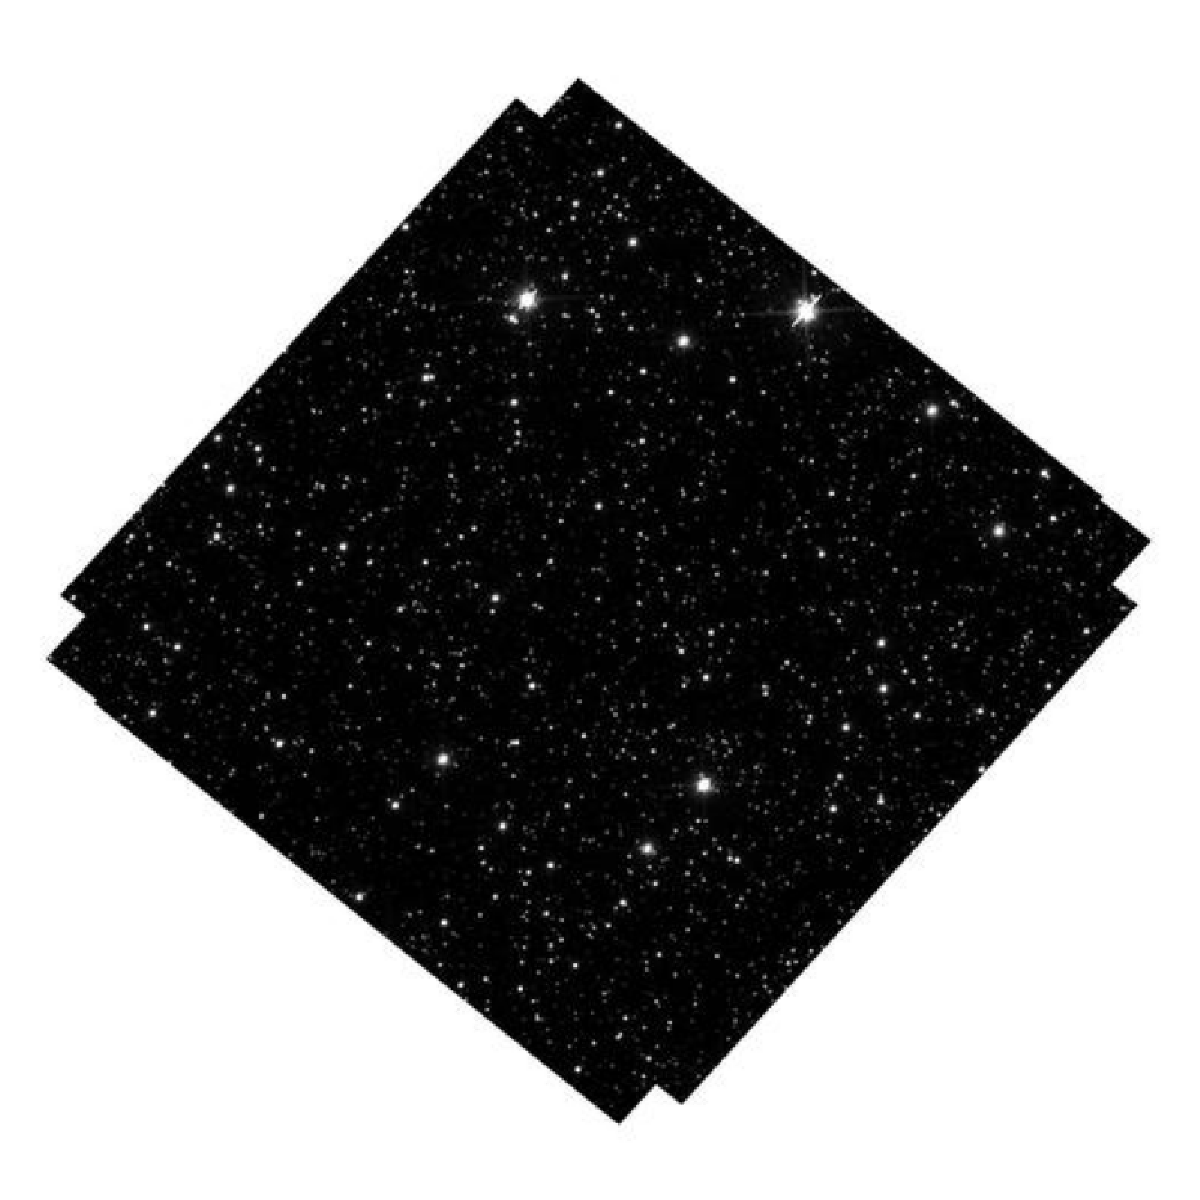
\includegraphics[width=0.2\textwidth]{\thedatafolder/img_0.pdf} & \centering \input{\thedatafolder/cycle_0.txt} & \centering \input{\thedatafolder/id_0.txt} &  {\scriptsize \input{\thedatafolder/sum_0.txt}} \tabularnewline
          \midrule
          \centering 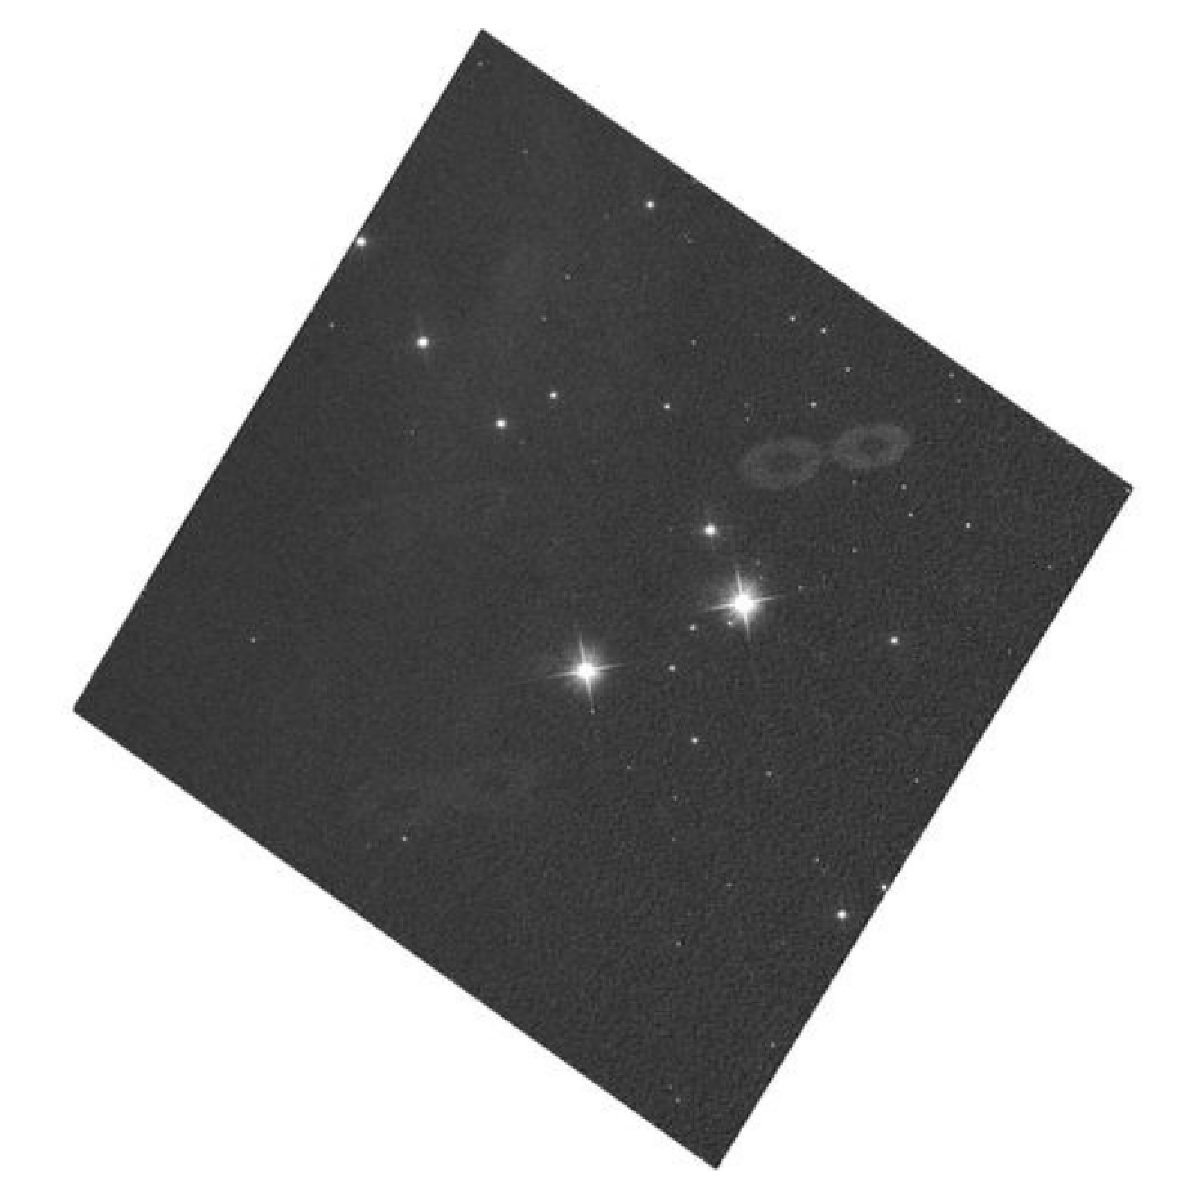
\includegraphics[width=0.2\textwidth]{\thedatafolder/img_1.pdf} & \centering \input{\thedatafolder/cycle_1.txt} & \centering \input{\thedatafolder/id_1.txt} &  {\scriptsize \input{\thedatafolder/sum_1.txt}} \tabularnewline
          \midrule
          \centering 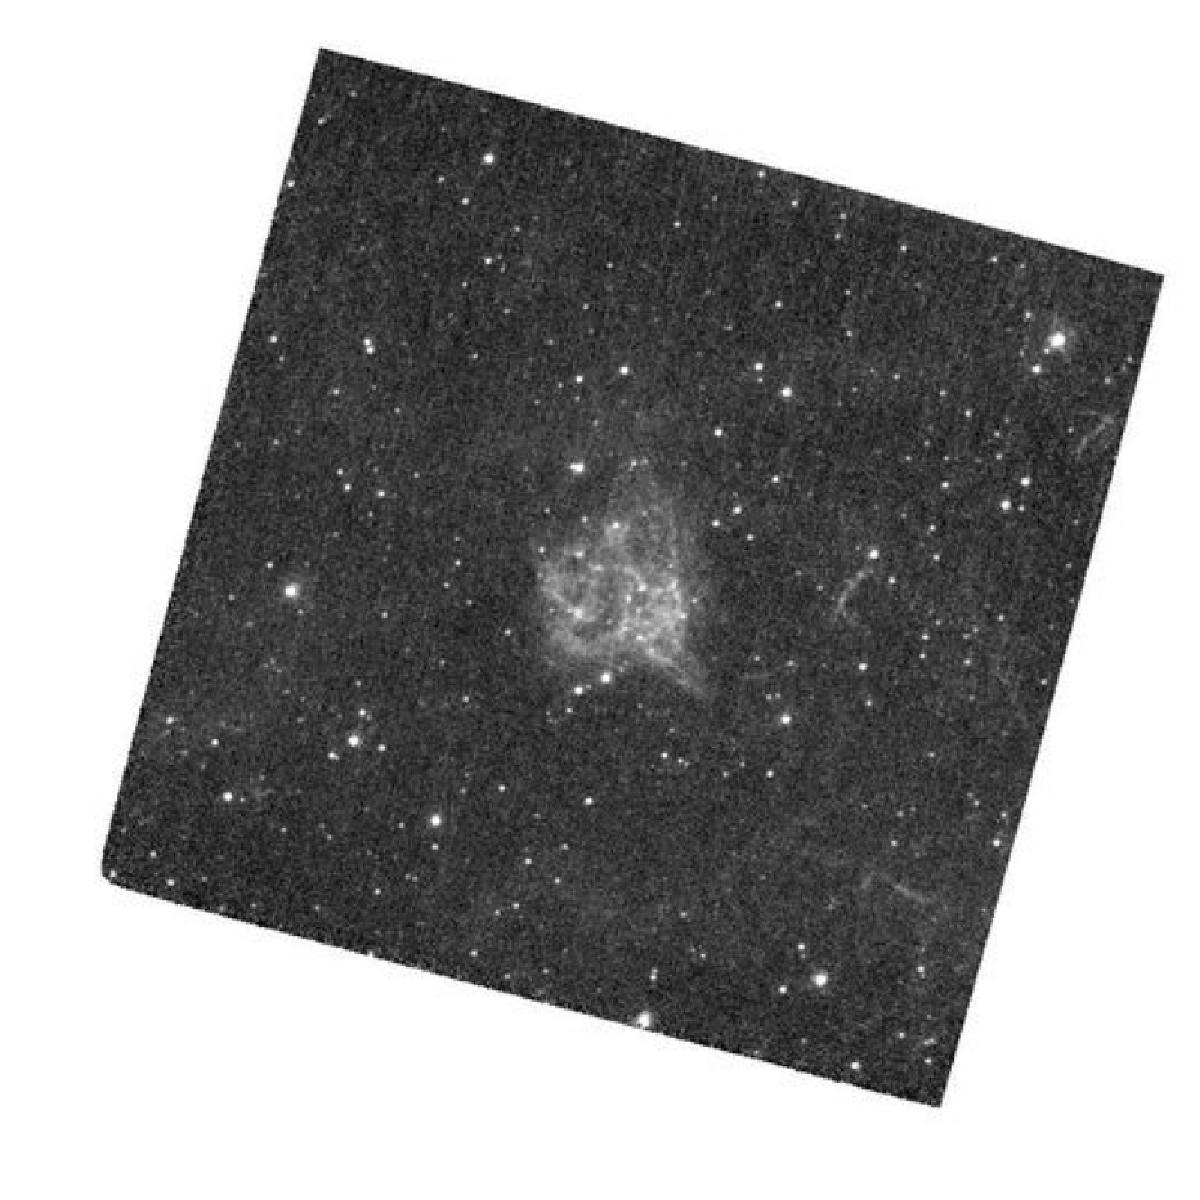
\includegraphics[width=0.2\textwidth]{\thedatafolder/img_2.pdf} & \centering \input{\thedatafolder/cycle_2.txt} & \centering \input{\thedatafolder/id_2.txt} &  {\scriptsize \input{\thedatafolder/sum_2.txt}} \tabularnewline
          \midrule
          \centering 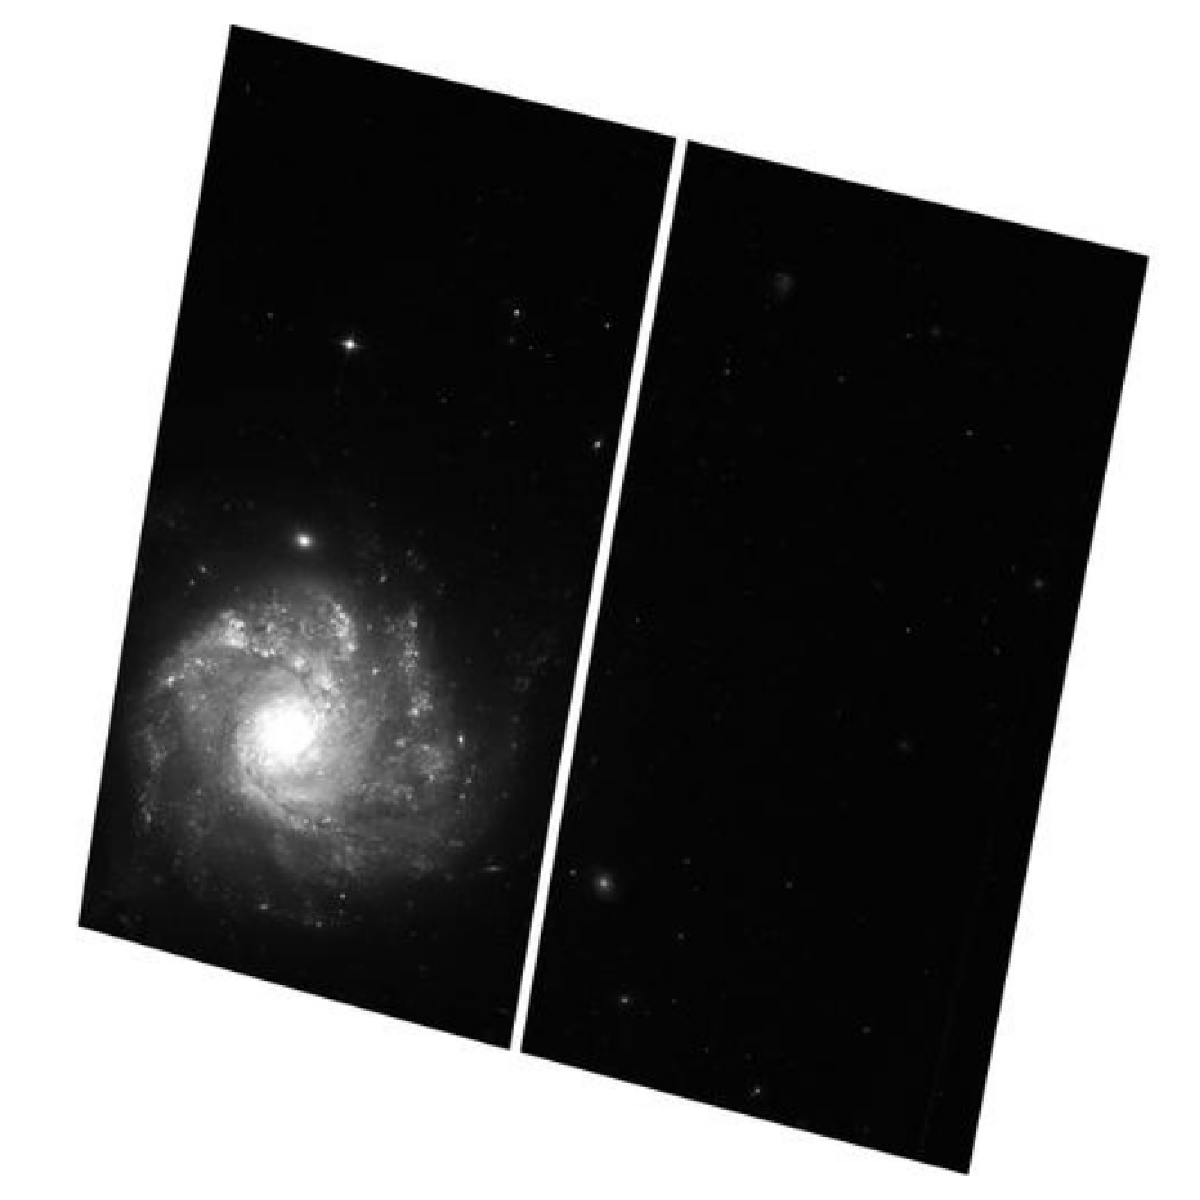
\includegraphics[width=0.2\textwidth]{\thedatafolder/img_3.pdf} & \centering \input{\thedatafolder/cycle_3.txt} & \centering \input{\thedatafolder/id_3.txt} &  {\scriptsize \input{\thedatafolder/sum_3.txt}} \tabularnewline
          \bottomrule
      \end{tabular}
      \caption{Examples of images and corresponding captions, constructed using the LLM-extracted summaries.
%
The CLIP model is fine-tuned using these text-image associations.}
      \label{tab:dataset}
  \end{table}

\begin{landscape}
      \begin{table}[h!]
          \centering
          \begin{tabular}{m{1.8cm} m{8cm} m{5cm} m{6cm}}
              \toprule
              \bfseries Prop. ID & \centering\arraybackslash \bfseries Proposal abstract & \multicolumn{2}{c}{\bfseries LLM-extracted summary} \tabularnewline
              \cmidrule(r){3-4}
              & & \centering\arraybackslash \bfseries Objects and phenomena & \centering\arraybackslash \bfseries Science use cases \tabularnewline
              \midrule
              \input{\thedatafolder/id1_0.txt} & {\scriptsize \input{\thedatafolder/abs1_0.txt}} & {\scriptsize \input{\thedatafolder/obj1_0.txt}} & {\scriptsize \input{\thedatafolder/sci1_0.txt}} \tabularnewline
              \midrule
              \input{\thedatafolder/id1_1.txt} & {\scriptsize \input{\thedatafolder/abs1_1.txt}} & {\scriptsize \input{\thedatafolder/obj1_1.txt}} & {\scriptsize \input{\thedatafolder/sci1_1.txt}} \tabularnewline
              \midrule
              \input{\thedatafolder/id1_2.txt} & {\scriptsize \input{\thedatafolder/abs1_2.txt}} & {\scriptsize \input{\thedatafolder/obj1_2.txt}} & {\scriptsize \input{\thedatafolder/sci1_2.txt}} \tabularnewline
              \midrule
              \input{\thedatafolder/id1_3.txt} & {\scriptsize \input{\thedatafolder/abs1_3.txt}} & {\scriptsize \input{\thedatafolder/obj1_3.txt}} & {\scriptsize \input{\thedatafolder/sci1_3.txt}} \tabularnewline
              \bottomrule
          \end{tabular}
          \caption{Examples of the initial parts of raw proposal abstracts (second column) and LLM (\textsc{Mixtral-8x7B})-extracted summaries (rightmost two columns), separately extracting objects and phenomena as well as potential downstream science use cases.}
          \label{tab:datasetsumm}
      \end{table}
  \end{landscape}

\section{Methodology}
\label{sec:methodology}

Our goal is to learn a semantically  meaningful joint representation between HST observation images and natural language.
%
We leverage the strong generalization capabilities demonstrated by pre-trained CLIP models and adapt these to work with domain-specific \hubble data via fine tuning.

\paragraph*{Pre-trained CLIP model}

CLIP \citep[Contrastive Language-Image Pretraining;][]{radford2021learning} is a multi-modal model pre-trained on a large corpus of image-text pairs via weak supervision using a contrastive loss.
%
Given a minibatch $\mathcal{B}$ of $|\mathcal{B}|$ image-text pairs $\{(I_i, T_i)\}$, the goal is to align the learned representations of corresponding (positive) pairs $(I_i, T_i)$ while repelling the representations of unaligned (negative) pairs $(I_i, T_{j\neq i})$.
%
Image and text encoders $f: I \rightarrow \mathbb R^{n_\text{emb}}$ and $g: T \rightarrow \mathbb R^{n_\text{emb}}$ are used to map images and text to a common embedding space of dimension $n_\text{emb}$.
%
The standard softmax-based bidirectional variation of the InfoNCE~\citep{oord2018representation} contrastive loss function was introduce for training CLIP-style architectures \citep{radford2021learning}
\begin{equation}
  \mathcal{L}(\mathcal{B})=-\frac{1}{2|\mathcal{B}|} \sum_{i=1}^{|\mathcal{B}|}\left(\log \frac{e^{x_i \cdot y_i / \tau}}{\sum_{j=1}^{|\mathcal{B}|} e^{x_i \cdot y_j / \tau}}+\log \frac{e^{x_i \cdot y_i / \tau}}{\sum_{j=1}^{|\mathcal{B}|} e^{x_j \cdot y_i / \tau}}\right)\label{eq:softmax_loss}
\end{equation}
where ${x}_i={f\left(I_i\right)}/{\left\|f\left(I_i\right)\right\|}$ and ${y}_i={g\left(T_i\right)}/{\left\|g\left(T_i\right)\right\|}$ are the normalized representations of the $i$-th image and text, respectively, and $\tau$ is a learnable temperature hyperparameter.
%
Note that this loss treats the image and text representations symmetrically, ensuring that the two modalities are on the same footing.

We use the CLIP-ViT-B/16 \citep{radford2021learning} variant as the base pre-trained CLIP model.
%
This model uses a 12-layer, 12-head, 768-embedding dimension vision transformer as the image encoder and a 12-layer, 8-head, 512-embedding dimension sequence transformer as the text backbone.
%
The text encoder has a maximum length of 77 tokens and the image encoder a native resolution of $224\times224$.
%
Linear projection layers map the outputs of the image and text encoders to a common embedding space of dimension $n_\text{emb}=512$.
%
In total, the model has 149,620,737 trainable parameters.
%
The model was originally trained on 400 million image-text pairs from internet data.
%


\paragraph*{Fine-tuning procedure}

The base CLIP model is fine-tuned using the dataset described in Sec.~\ref{sec:dataset}, using either the LLM-summarized data, the raw proposal abstracts, or single-concept summaries.
%
When using raw proposal abstracts, random chunks of the text delimited by periods are selected on the fly to fit within the maximum token length of the text encoder.
%
Images are randomly cropped to the native resolution of the image encoder and randomly rotated at each training step.
%
Given the relatively modest size of the fine-tuning set, a batch size $|\mathcal B| = 32$ is used throughout; larger batch sizes were seen to be susceptible to overfitting.
%
We note that the positive and negative image-text association is noisy and imperfect, since multiple images can be associated with the same abstract.

We explore three different methods of training the model on our domain dataset: \emph{(1)} Fine-tuning the entire network, starting from the pre-trained base model; \emph{(2)} Freezing the base image and text encoders, and training a small projection head; and \emph{(3)} Training the entire model from scratch.
%
For \emph{(2)}, we use a 2-layer MLP with 1024 units and a GELU activation layer, projecting onto the 512-dimensional embedding space.

Models were trained over 20,000 steps with 2000 linear warmup steps 
% and cosine decay 
using the AdamW optimizer \citep{DBLP:conf/iclr/LoshchilovH19,DBLP:journals/corr/KingmaB14} with  %peak 
learning rate of $10^{-5}$ and weight decay $10^{-3}$.
%
Training takes approximately 3 hours on 4 Nvidia A100 GPUs.
Models were instantiated and trained using the \package{Jax} \citep{jax2018github} ecosystem.
%


\paragraph*{Evaluation}

The model is evaluated by tracking the loss in Eq.~\ref{eq:softmax_loss} as well as the top-$k\%$ retrieval accuracy on the held out validation set over the course of training.
%
The retrieval accuracy is defined as the fraction of associated captions which fall within the top $k\%$ of captions by cosine similarity of the normalized embeddings $x_i \cdot y_j$, averaged over the images in the validation set.

We also qualitatively evaluate the learned embeddings through image retrieval (i.e., retrieving the most relevant images from a set using natural language queries) and description retrieval (i.e., querying the astrophysical object classes and science use cases most relevant to a given observation) experiments.

\section{Results and Discussion}
\label{sec:results}

\paragraph*{Validation metrics}

Figure~\ref{fig:retrieval_acc} shows the contrastive loss (left) and the top-10\% retrieval accuracy on the held out validation set over the course of training, for different training configurations considered.
%
The purple lines show the metrics evaluated when training with batches where the image-text associations are randomly shuffled, serving as a baseline.
%
This baseline is seen to do on par with random expectation, unlike the others, validating the presence of a significant association signal between images and text in the dataset.
%
Interestingly, the base pre-trained model performs better than random expectation, with a top-10\% retrieval accuracy of $\sim 15\%$.
%
We therefore compare the qualitative performance of the base model with the fine-tuned model on downstream retrieval tasks.

The model with LLM-guided summarization (yellow lines) is seen to perform on-par with the model using raw abstracts as captions (orange line), despite the stronger association signal in the summarized dataset curated.
%
Fine-tuning a small MLP head over frozen vision and text backbones (green lines), training from scratch (blue lines), and using the single-concept summaries (red lines) show a non-trivial improvement compared to the random baseline as well as base model, but with deteriorated performance compared to fine-tuning with either summarized or raw abstracts.

\begin{figure*}[!h]
  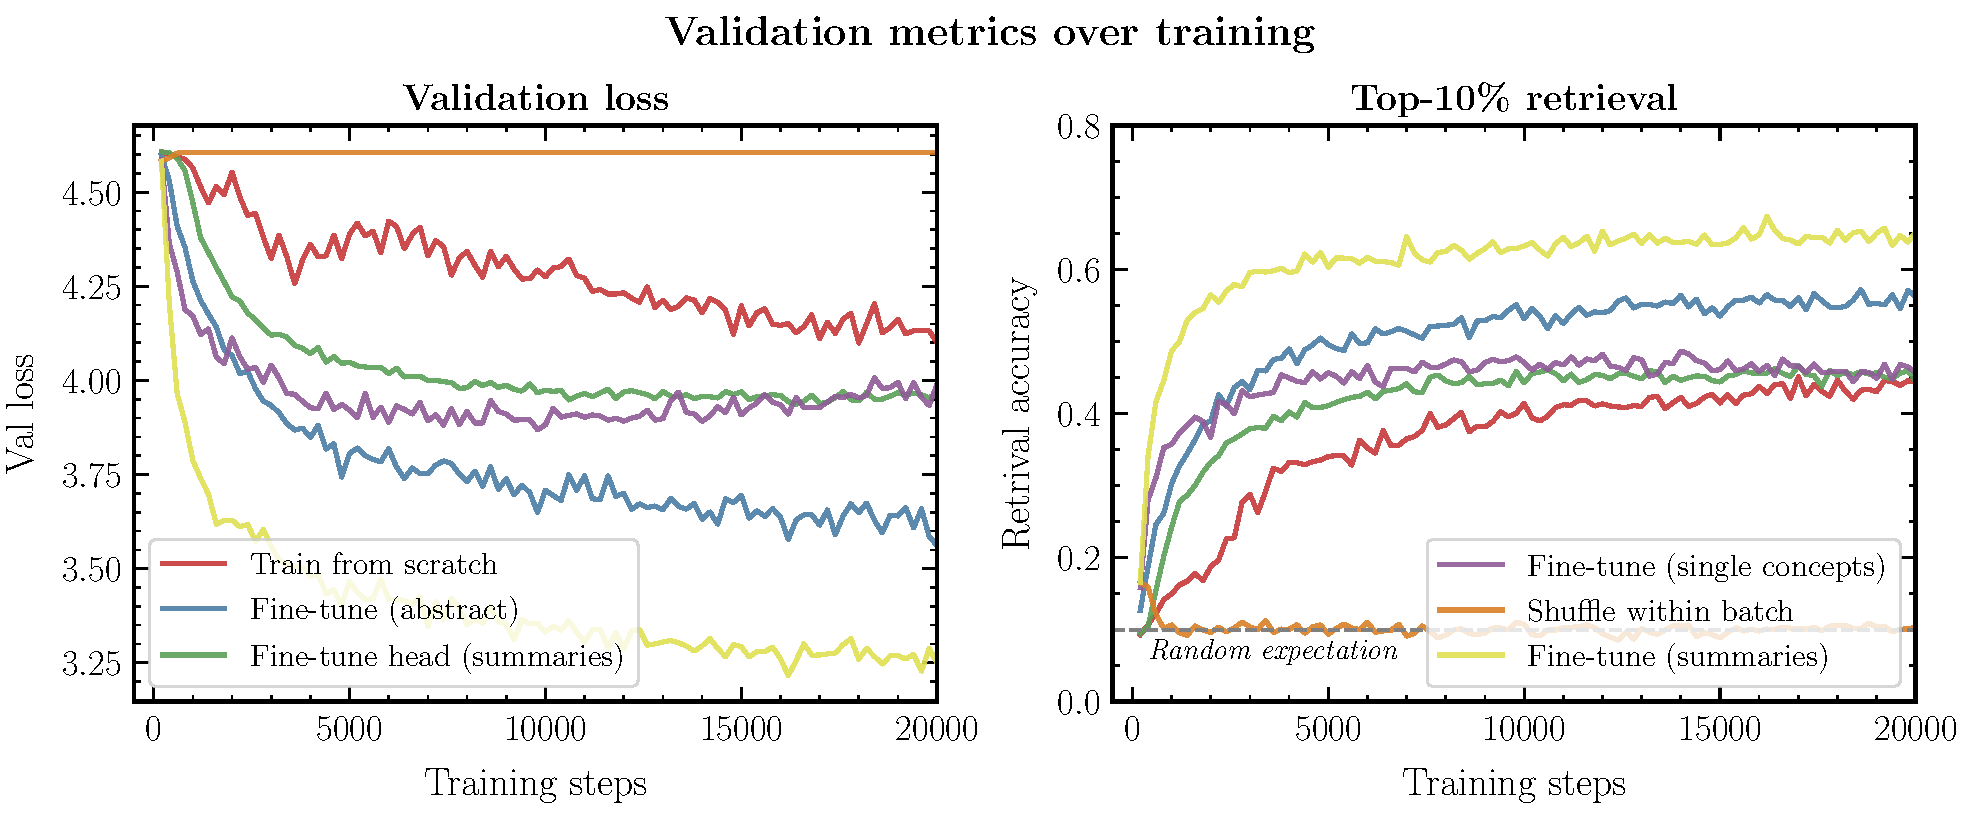
\includegraphics[width=0.95\textwidth]{plots/val_metrics.pdf}
  \caption{The CLIP contrastive loss from Eq.~\ref{eq:softmax_loss} (left) and the top-10\% retrieval accuracy (right) computed on the validation set over the course of training. Shown for the dataset with summarized abstracts (orange), dataset using raw proposal abstracts (yellow), dataset with single-concept summaries (red), only fine-tuning a small MLP head (green), training from scratch (blue), and trained with shuffled image-text pairs (purple).}
  \label{fig:retrieval_acc}
  \end{figure*}

\paragraph*{Image retrieval}

Having aligned the image and text representations, we can query the validation set using natural language and show the most `relevant' images when ranked by cosine similarity.
%
We show these in Figs.~\ref{fig:tti_base} and \ref{fig:tti} for the base model and fine-tuned model respectively using four simple curated queries: `jupiter', `dwarf galaxy', `SN1987A' (a specific, prominent supernova), and `strong lensing'.

While the base model shows some signs of meaningful retrieval (e.g., the image of jupiter in the first row of Fig.~\ref{fig:tti_base}, and images of galaxies in the second row), it is challenging to discern meaningful strong associations between the retrieved images and corresponding query.

The fine-tuned model (Fig.~\ref{fig:tti}), meanwhile, shows strikingly different behavior.
%

% For example, it is able to return images with processing and assembly artifacts particular to HST (e.g., the lines through the middle in some images), which typically receive low similarity scores when using the base model.
%

Images of Jupiter are returned for the `jupiter' query, with the planet visible in all four images.
The `dwarf galaxy' images correspond to proposals aiming to measure the kinematics of the stellar cores of dwarf galaxies.
%
Supernova SN1987 itself can be seen in the most relevant images for the `SN1987A' query, with the fourth image corresponding to a supernova remnant.
%
Cluster-scale as well as galaxy-scale gravitational lenses are returned by the `strong lensing' query, with lensing patterns visible in the images.

\paragraph*{Text retrieval}

We can use images from the validation set as queries and retrieve the most relevant text chunks (e.g., contained objects and use cases) from a curated list.
%
We show the result of image-to-text retrieval in Fig.~\ref{fig:itt}, for the base as well as fine-tuned models, using four observations from the validation set.
%
We curate a list of possible text associations by querying the \textsc{Claude}\footnote{\url{https://claude.ai/}} large language model for such a list, which we show in App.~\ref{app:categories}.

The top four text associations are shown for each image query.
%
The `ground truth' summarized abstract is shown in the right column.
%
The base as well as fine-tuned models are seen to return a mix of relevant and less-relevant associations, although showing different qualitative behavior.
%

The second row (supernova 1987A) highlights an interesting pattern -- the base model erroneously attributes the object at the center of the image to a gravitational lens, while the fine-tuned model correctly identifies it as a supernova remnant.

\paragraph*{Statistical distributions on the validation set}

Figure~\ref{fig:sim_valtrain} (top left) shows the distribution of cosine similarities between corresponding image and text embeddings, $x_i$ and $y_i$, for the LLM-summarized abstracts using the fine-tuned CLIP model (red line), and for the base CLIP model (blue line).
%
Distributions after shuffling the order of text embeddings -- therefore randomizing the image-text correspondence -- are shown as dashed lines.
%
The distributions for the base model is seen to be sharply peaked at a specific value, showing little diversity and being very similar between the shuffled (dashed blue) and non-shuffled (solid blue) versions.
%
Histograms for the fine-tuned model, on the other hand, show a clear separation between the shuffled and corresponding text-image pair versions.

Similarly, Fig.~\ref{fig:sim_valtrain} (top right) shows the distribution of cosine similarities between corresponding image-text pairs for the single-concept captions (solid red) and the shuffled versions (dashed red).
%
The distribution for corresponding pairs is only modestly shifted compared to the shuffled version, indicating that assigning $\mathcal O(400)$ labels to the images using an LLM results in a weaker association signal compared to using noisy captions.
%
The purple line shows the distribution of cosine similarities between corresponding pairs with single-concept summaries, but evaluated using a model trained on the LLM-summarized abstracts.
%
This distribution is more skewed towards higher similarity values, indicating that the model trained on diverse caption can still better capture the association signal in the single-concept summaries compared to one trained specifically using the single-concept summaries.

Finally, Fig.~\ref{fig:sim_valtrain} (bottom) shows the image-to-text retrieval accuracy -- i.e., the fraction of correct abstracts which fall within the top $k$-fraction of captions by cosine similarity, averaged over images in the validation set -- as a function of the retrieval fraction $k$.
%
In this case, we evaluate three models -- fine tuned on raw abstracts (red), fine-tuned on LLM-summarized abstracts (blue), and fine-tuned on single-concept summaries (green), and the base model (purple) -- on the summarized abstracts.
%
Remarkably, the model trained on raw abstracts shows very similar performance on the summarized abstracts compared to that trained on the summarized abstracts themselves, indicating that \emph{(1)} the association signal is preserved in the summarization process, and \emph{(2)} the model is able to effectively leverage meaningful concepts in the noisy raw abstracts through weak supervision.


\begin{figure*}[!h]
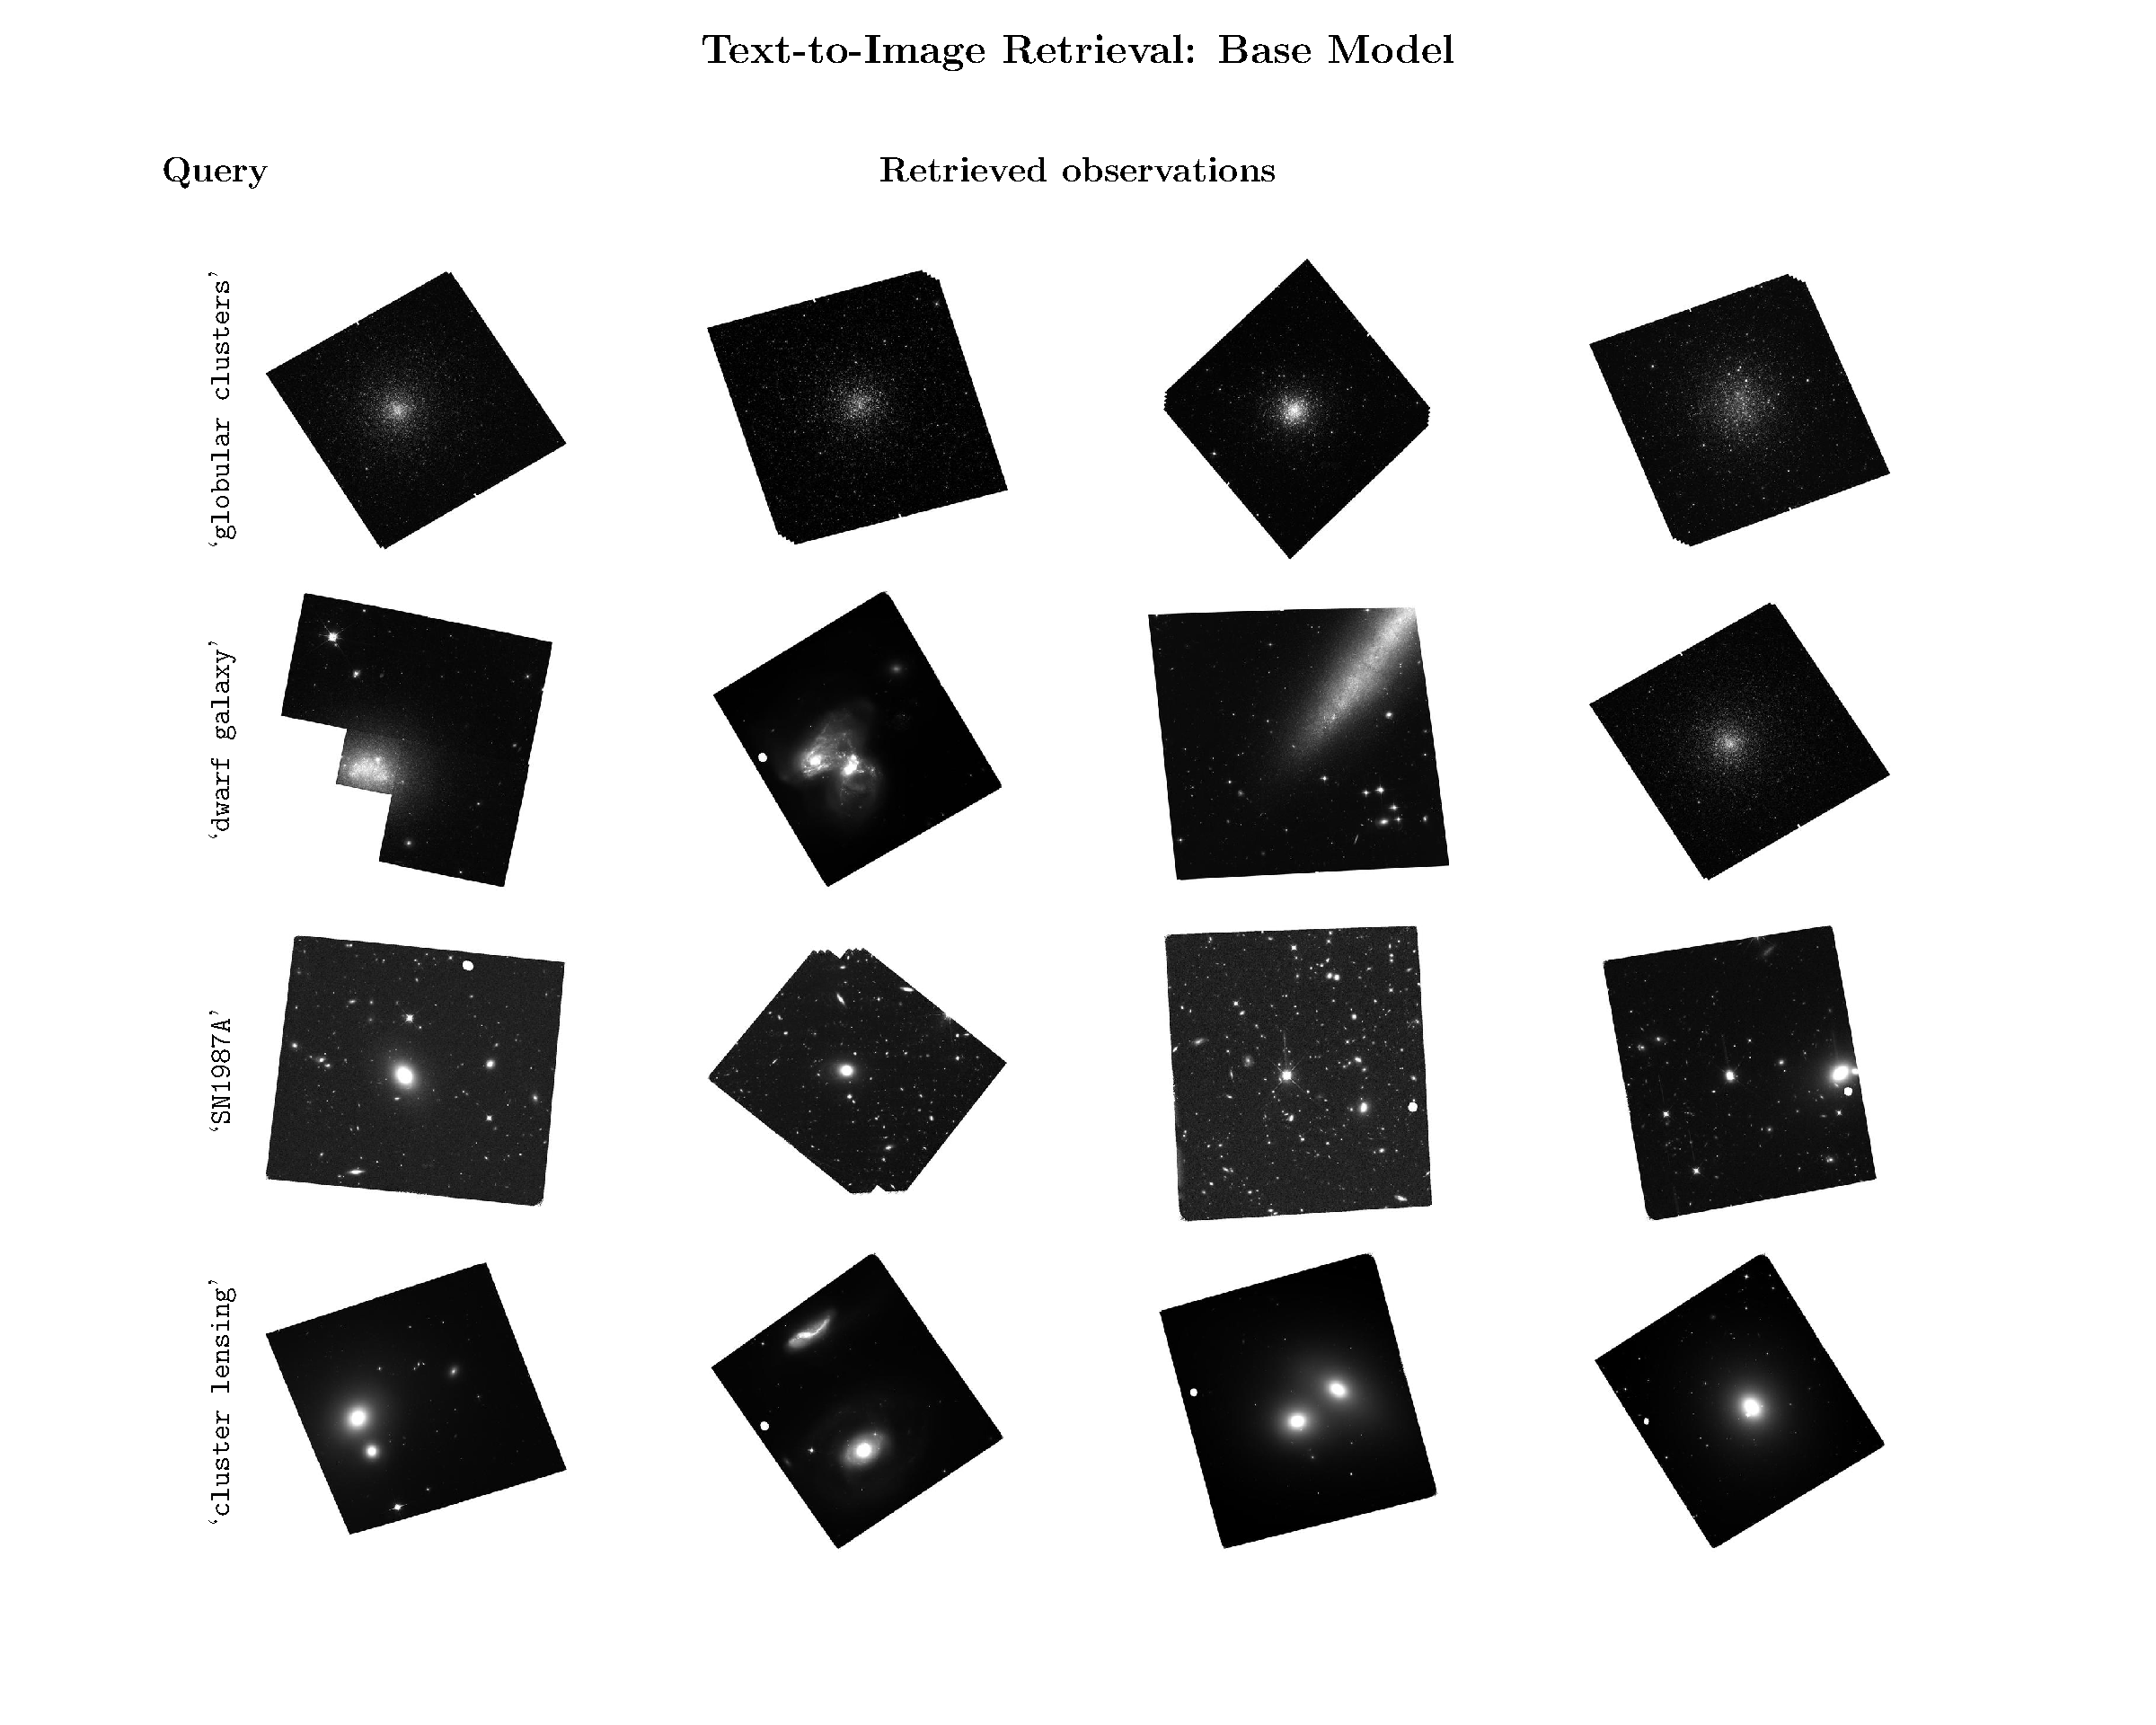
\includegraphics[width=0.95\textwidth]{plots/tti_base.pdf}
\caption{Image retrieval using the base CLIP model on four curated queries.}
\label{fig:tti_base}
\end{figure*}

\begin{figure*}[!h]
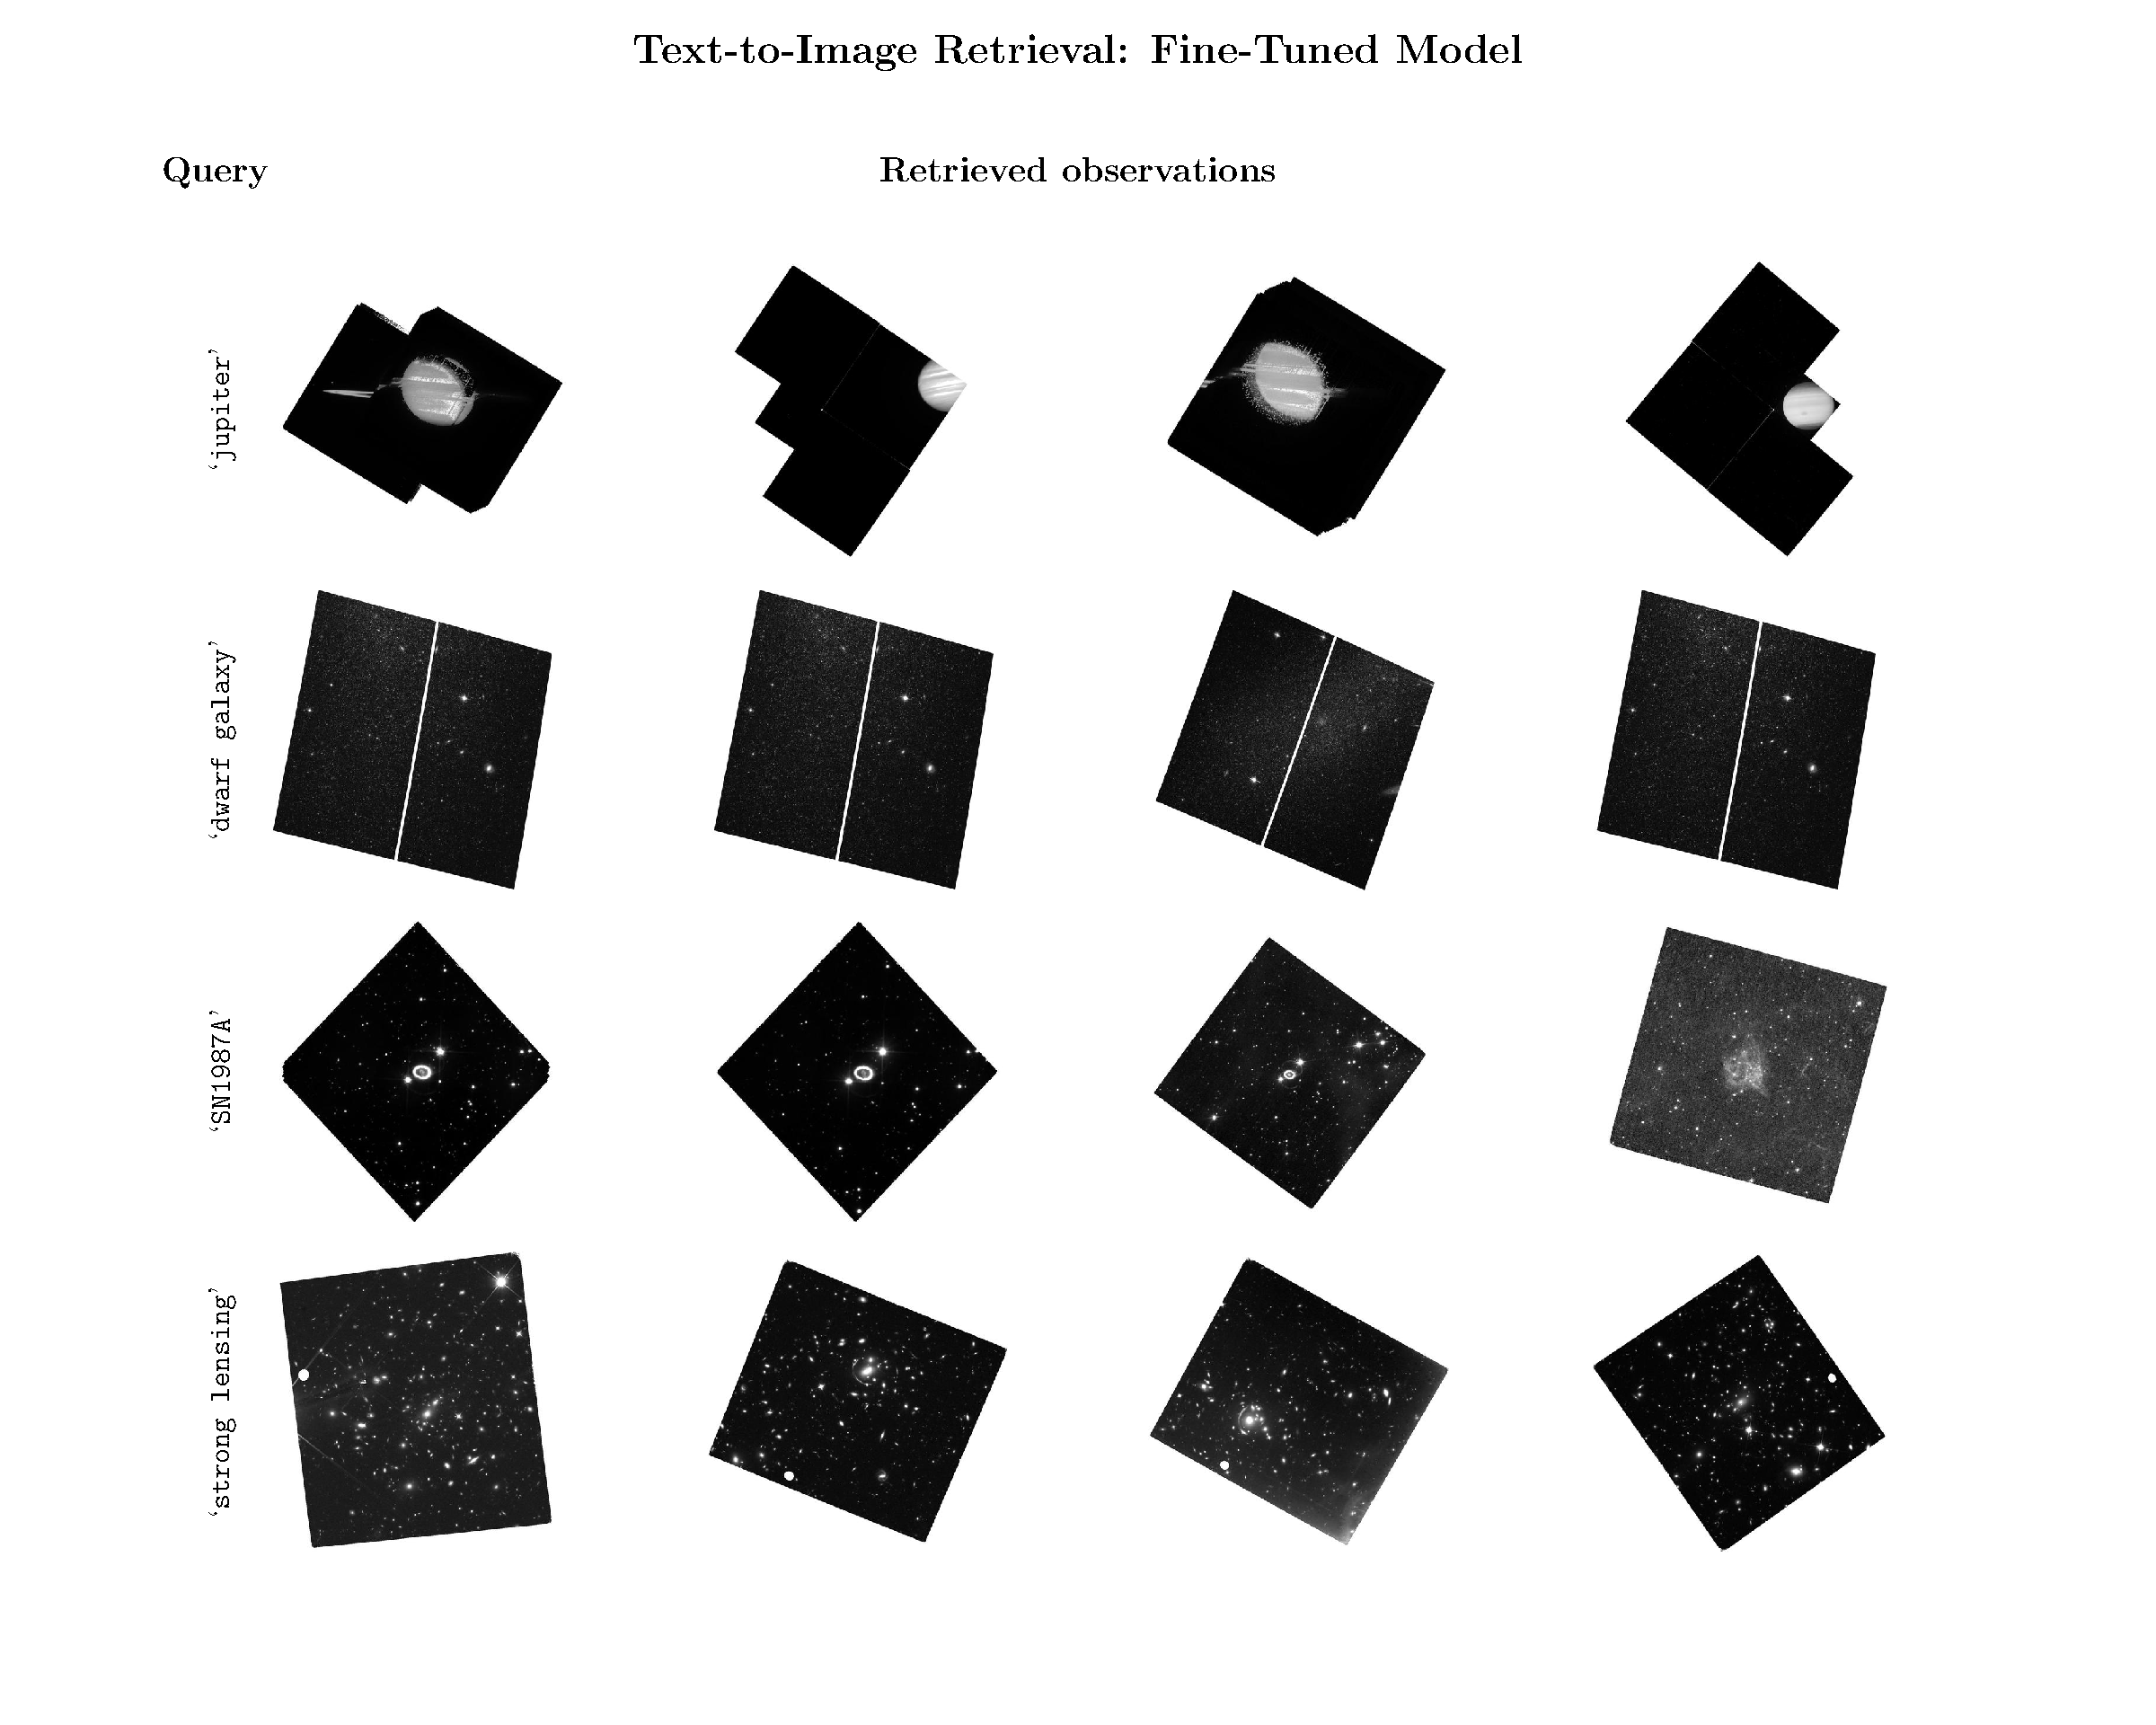
\includegraphics[width=0.95\textwidth]{plots/tti.pdf}
\caption{Image retrieval using the fine-tuned CLIP model on four curated queries.}
\label{fig:tti}
\end{figure*}

\begin{figure*}[!h]
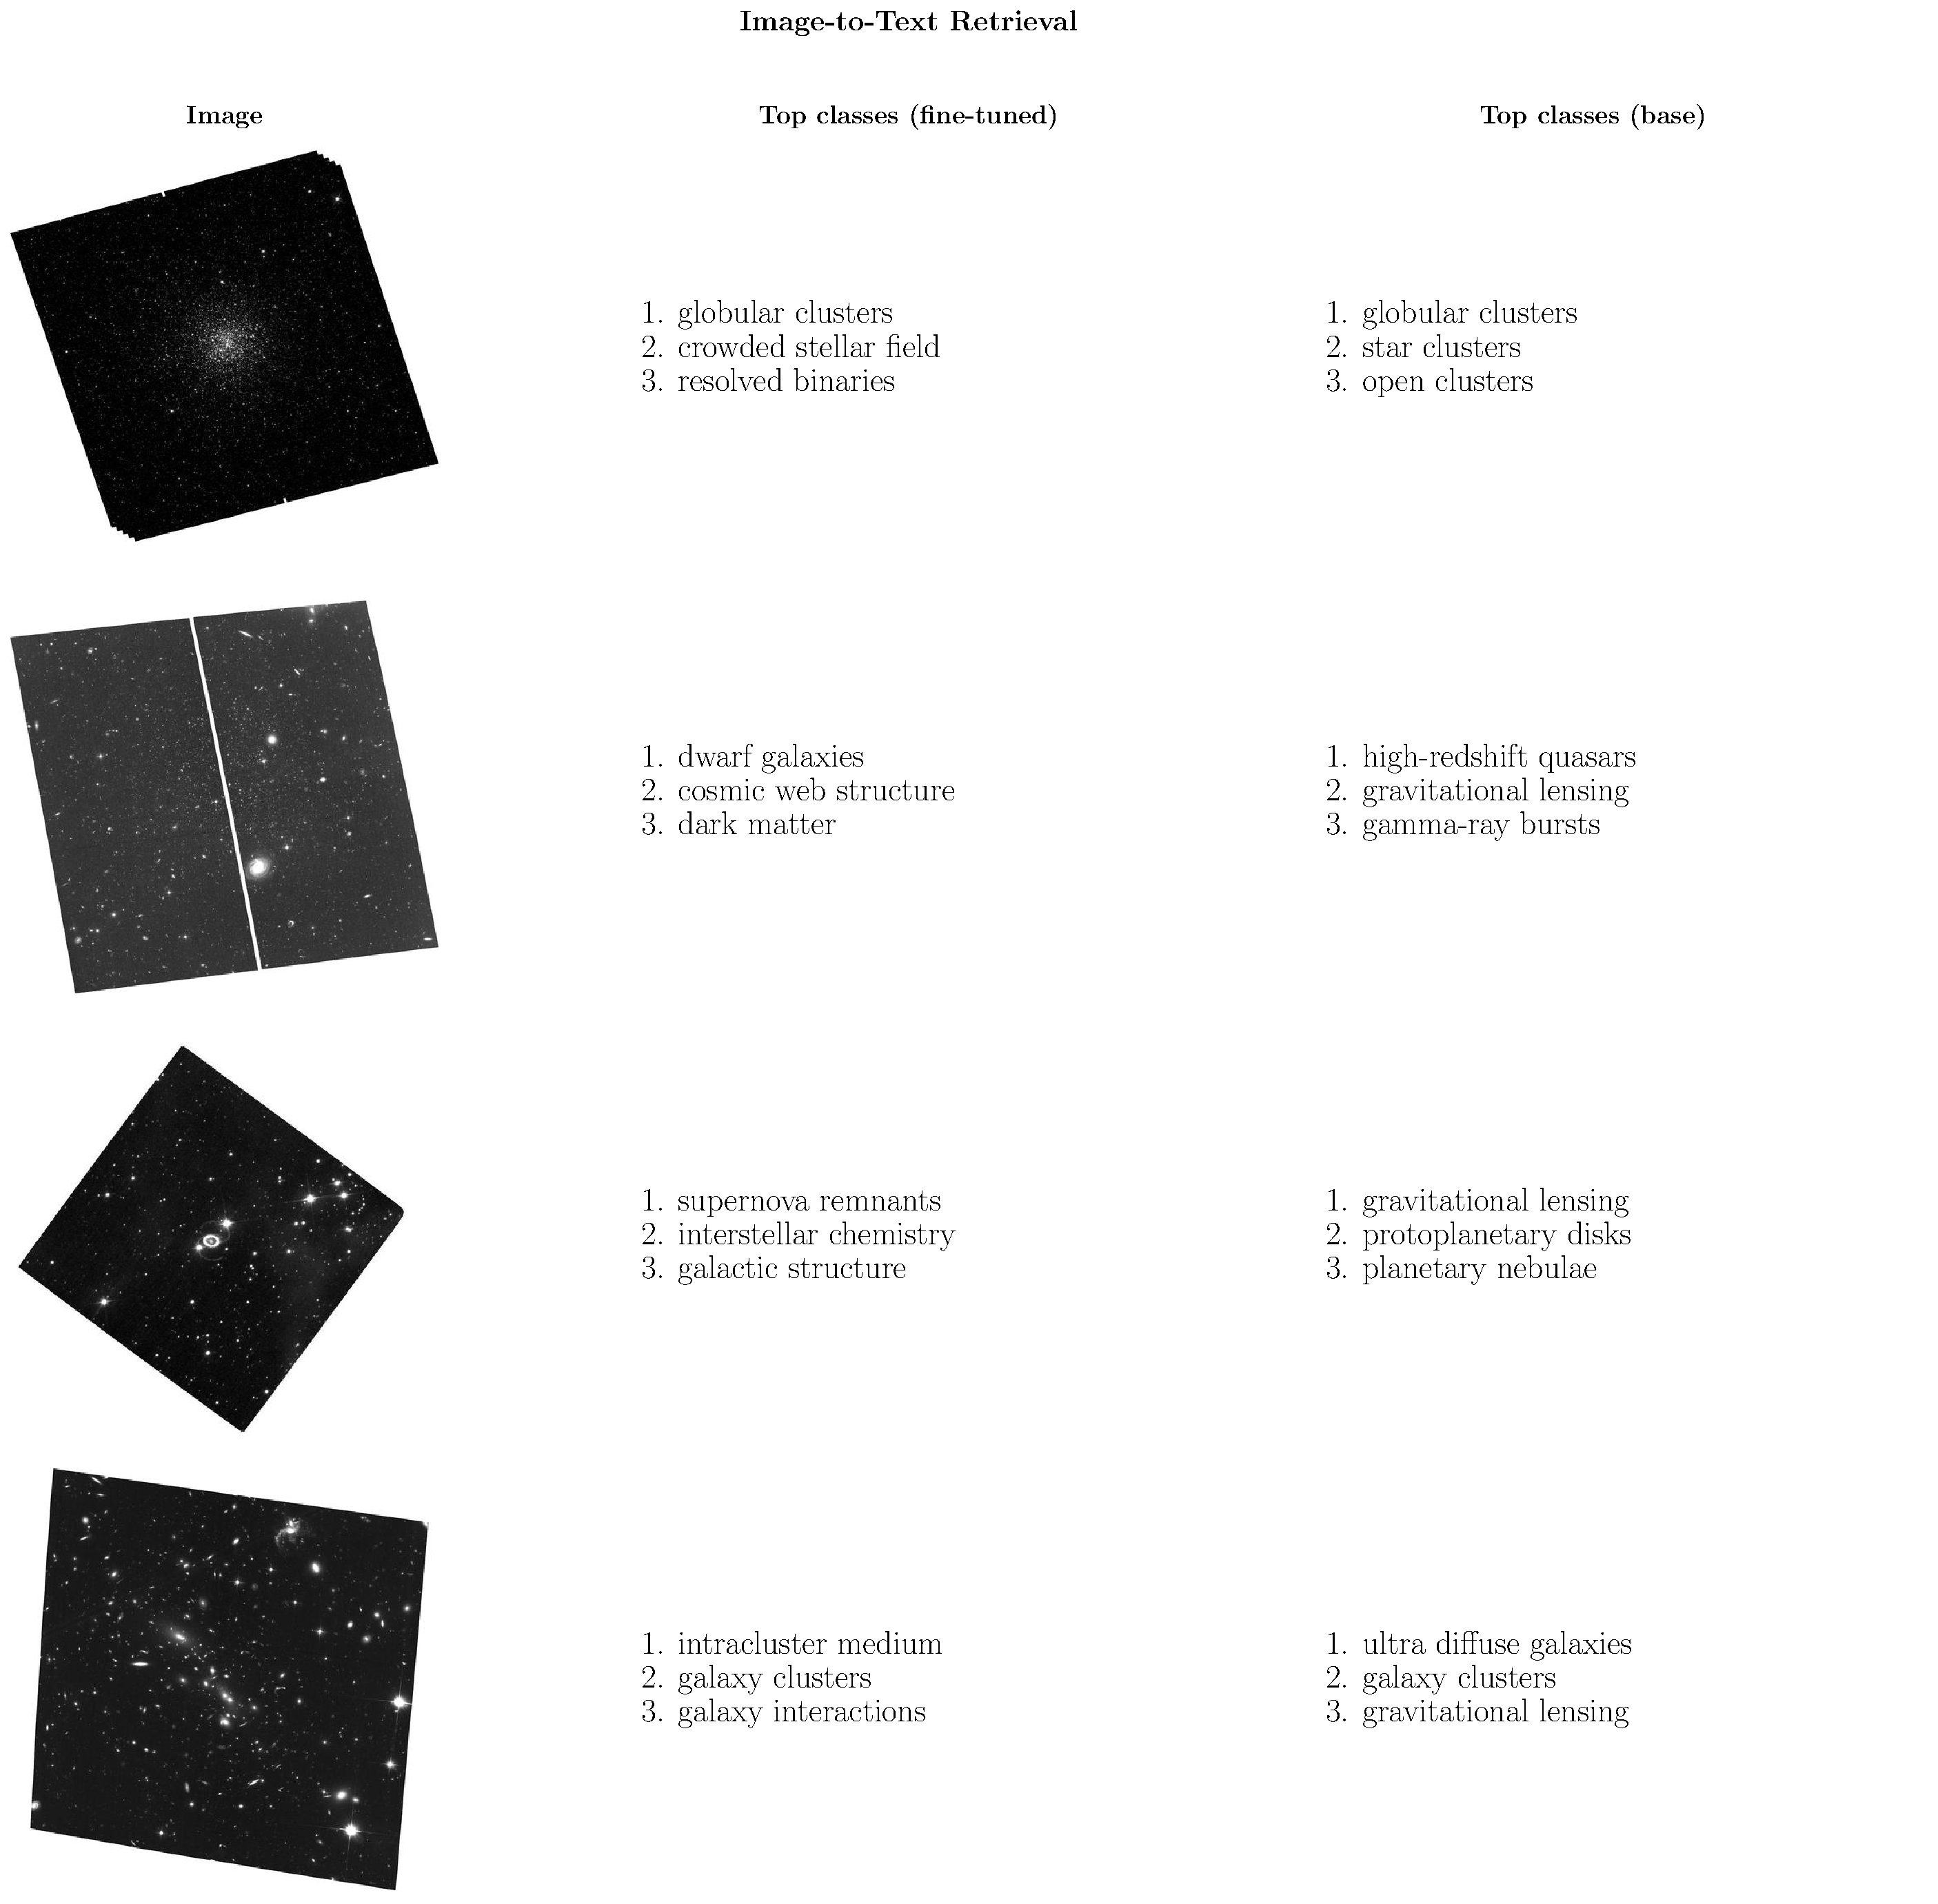
\includegraphics[width=0.95\textwidth]{plots/itt.pdf}
\caption{Text associations from a curated list most closely matching a given image query, for both the fine-tuned and base models. The `ground truth' LLM-summarized abstract is shown in the right column.}
\label{fig:itt}
\end{figure*}

\begin{figure*}[!h]
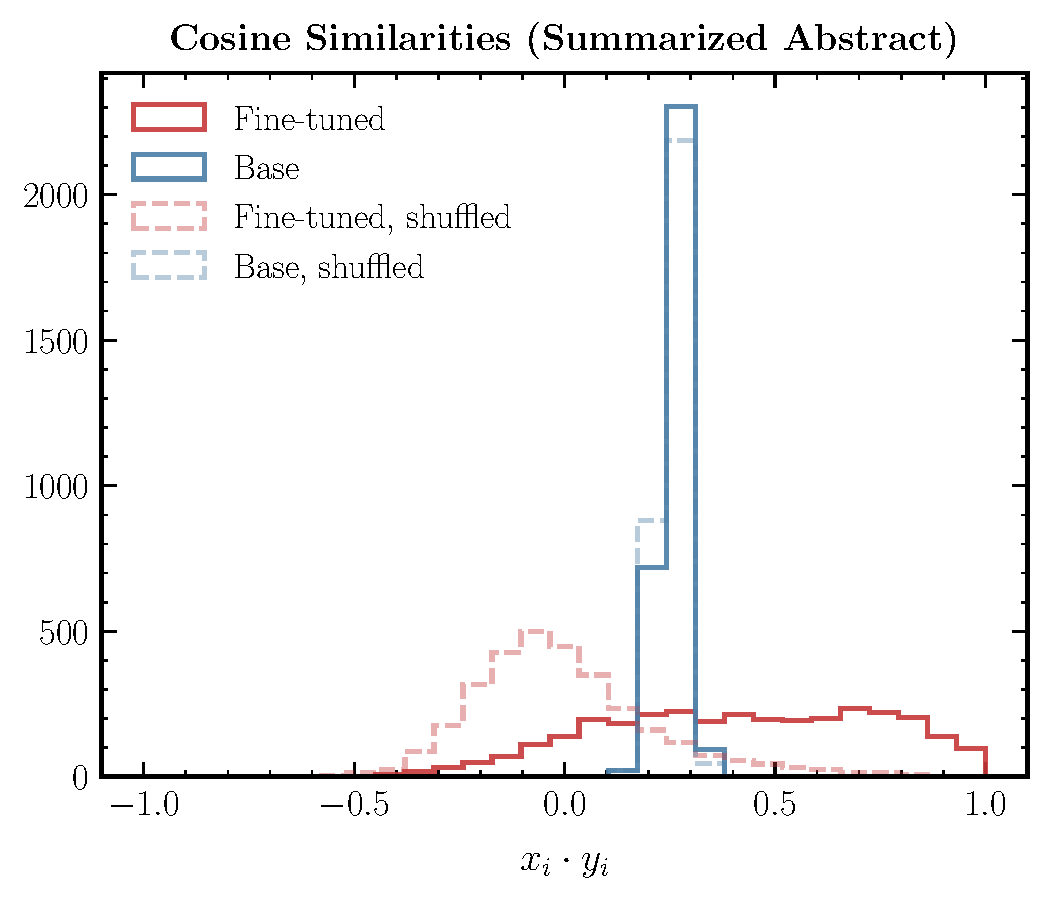
\includegraphics[width=0.45\textwidth]{plots/sim_val.pdf}
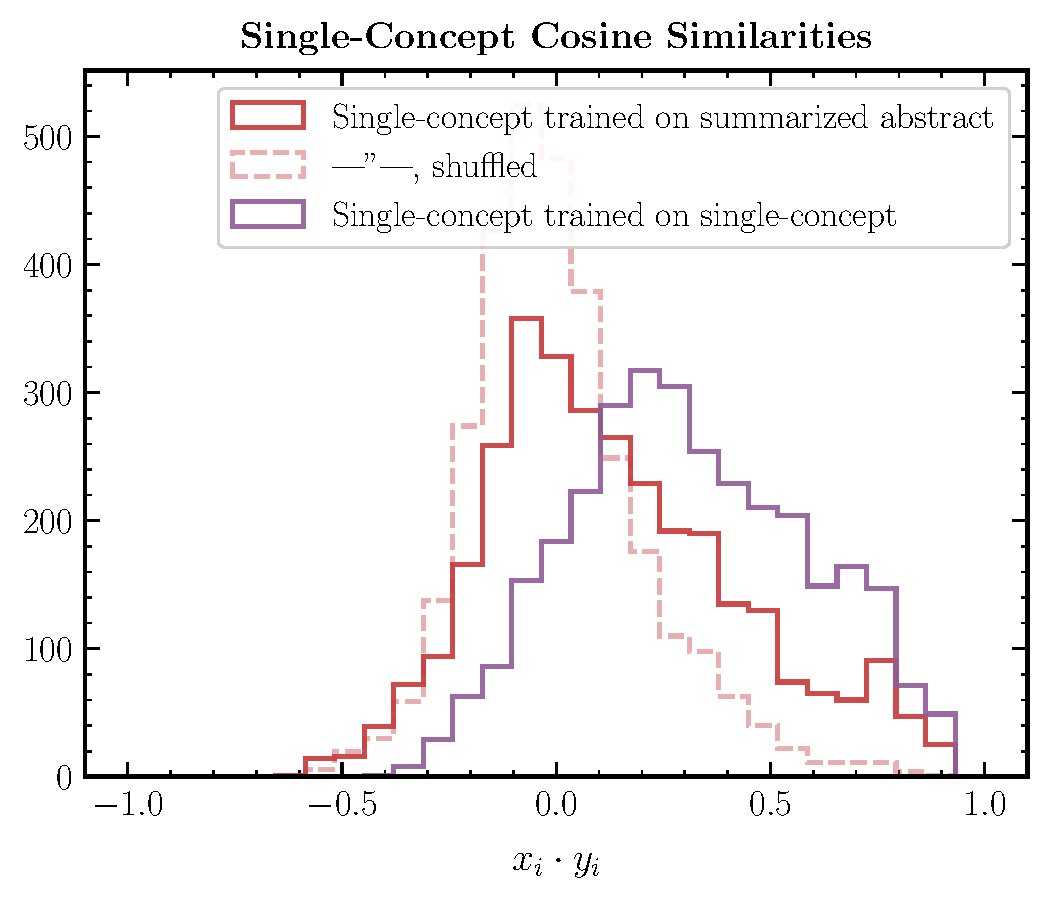
\includegraphics[width=0.45\textwidth]{plots/sim_summ1.pdf}
\centering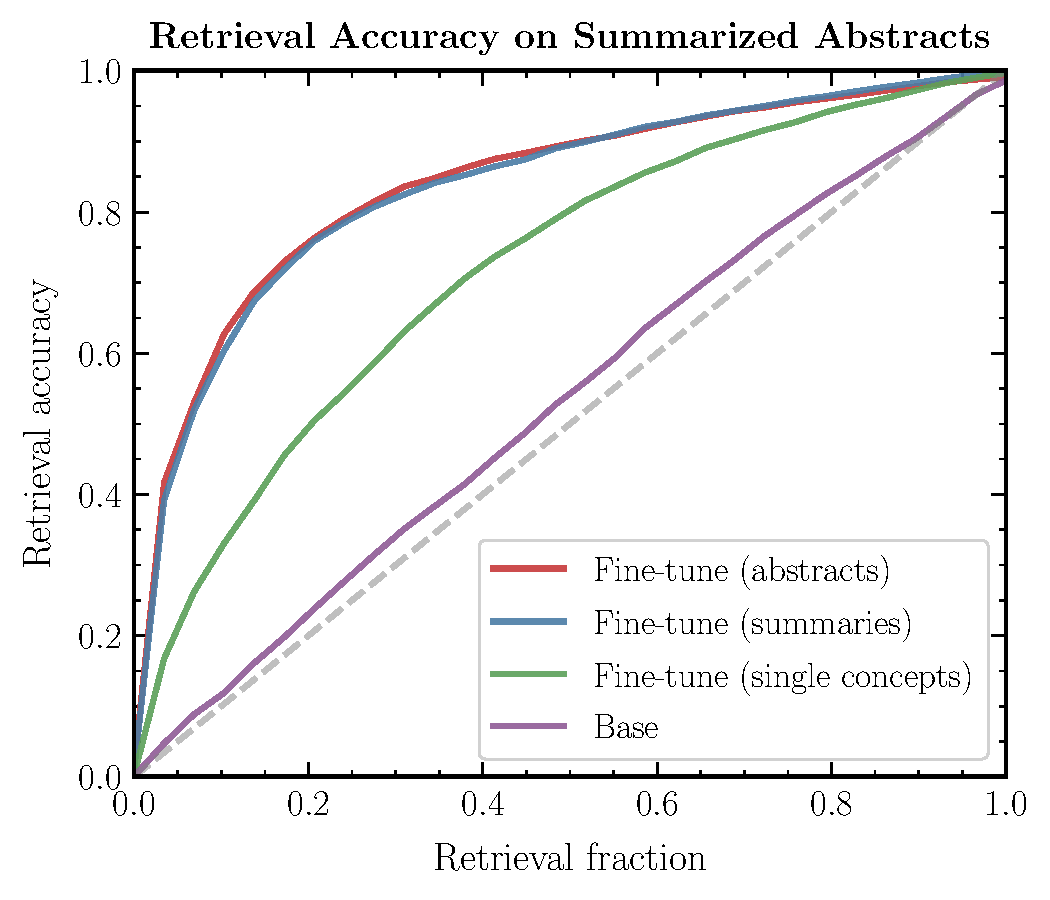
\includegraphics[width=0.45\textwidth]{plots/retrieval.pdf}
\caption{Distribution of cosine similarities between corresponding image and text embeddings, $x_i$ and $y_i$. (Top row) For the LLM-summarized abstracts using the fine-tuned CLIP model (red line), and for the base CLIP model (blue line), shown for (top left) the set of validation pairs and (top right) same number of training set pairs. Versions with the ordering of text embeddings shuffled are shown in dashed. (Bottom) For the single-concept summaries, when evaluated using the CLIP model fine-tuned on LLM-summarized abstracts (red) and fine-tuned on the single-concept summaries themselves (purple).}
\label{fig:sim_valtrain}
\end{figure*}

\section{Outlook and Conclusions}
\label{sec:conclusion}

We present \textsc{HubbleCLIP}, a multi-modal fountation model that associates observations imaged by the \hubble Space Telescope with natural language in a common, semantically-meaningful embedding space.
%
The model is fine-tuned from a pre-trained CLIP model on summarized versions of \hubble proposal abstracts, leveraging a noisy association signal between text and images.
%
We show that \textsc{HubbleCLIP} significantly outperforms the base CLIP model in quantitative metrics, such as retrieval accuracy, as well as quality of text-to-image and image-to-text retrieval.
%
We also introduce a novel LLM summarization process which leverages constrained generation to increase the association strength between images and captions while preserving salient information.
%
Overall, the procedure demonstrates the efficacy on fine-tuning generalist pre-trained models on small amounts of domain-specific data, in particular astronomical datasets.

Although the model explored here is fine-tuned using postage stamp images (i.e., preview-quality and not science-grade data), we highlight potential immediate as well as downstream use cases of this paradigm.
%
In particular, a robust model trained using weakly-supervised image-text pairs can be used to query survey data e.g., PHANGS~\citep{lee2022phangs}, COSMOS~\citep{scoville2007cosmic} using natural language, as well as to quickly find distinguishing patterns in such data that may not be apparent using specialized models or manual inspection.
%
The learned representations, having shown to correlate with physical characteristics of imaged objects, can also be fine-tuned via transfer learning to adapt to specific tasks e.g., classification~\citep{wei2020deep} or segmentation~\citep{hausen2020morpheus}.
%
Finally, while the CLIP model is restricted to retrieving nearest-neighbour associations within and across text/image modalities, the learned embeddings can be used as a starting point for training or fine-tuning multi-modal large-language models for interacting with survey data and receiving responses in natural language form, as well as grounding the responses based on an existing set of observations.

\paragraph*{Code and data availability}

The code, dataset, and fine-tuned models used in this work is available at \url{https://www.github.com/smsharma/HubbleCLIP}.

\paragraph*{Software}

This work relied on the \package{Astroquery} \citep{2019AJ....157...98G}, \package{BitsAndBytes} \citep{dettmers2022llmint8}, \package{Flax} \citep{flax2020github}, \package{Jax} \citep{jax2018github}, \package{Jupyter} \citep{Kluyver2016jupyter}, \package{Matplotlib} \citep{Hunter:2007}, \package{Numpy} \citep{harris2020array}, \package{Optax} \citep{deepmind2020jax}, \package{Outlines}, \package{Pandas} \citep{2020SciPy-NMeth}, \package{Pydantic}, \package{PyTorch} \citep{paszke2019pytorch}, \package{SciPy} \citep{2020SciPy-NMeth}, \package{Transformers} \citep{wolf2019huggingface}, and \package{Wandb} \citep{wandb} software packages.


% Code repo and package cites.
% Dataset availability

\paragraph*{Acknowledgments}

We thank Michael Brenner for helpful conversations.
%
This work is supported by the National Science Foundation under Cooperative Agreement PHY-2019786 (The NSF AI Institute for Artificial Intelligence and Fundamental Interactions, \url{http://iaifi.org/}).
%
This material is based upon work supported by the U.S. Department of Energy, Office of Science, Office of High Energy Physics of U.S. Department of Energy under grant Contract Number  DE-SC0012567. 
%
YS was supported by the Research Science Institute (RSI) program at MIT.
%
The computations in this paper were run on the FASRC Cannon cluster supported by the FAS Division of Science Research Computing Group at Harvard University.

This research is based on observations made with the NASA/ESA Hubble Space Telescope obtained from the Space Telescope Science Institute, which is operated by the Association of Universities for Research in Astronomy, Inc., under NASA contract NAS 5-26555.

Based on observations made with the NASA/ESA Hubble Space Telescope, and obtained from the Hubble Legacy Archive, which is a collaboration between the Space Telescope Science Institute (STScI/NASA), the Space Telescope European Coordinating Facility (ST-ECF/ESAC/ESA) and the Canadian Astronomy Data Centre (CADC/NRC/CSA).


\bibliography{main}
\bibliographystyle{tmlr}

\appendix
\section{Summarization via Regex-Guided Generation}
\label{app:guided-generation}

\SM{Technical description of regex-guided generation.}

\section{Prompts and Schema Used for Summarization}
\label{app:prompts}

We list here the prompts and schemata (i.e.
%
desired output formats) used at various stages for guided text generation via \package{Outlines} package interfacing with the \textsc{Mixtral-8x7B-Instruct} LLM.

\subsection{Abstract summarization into objects, phenomena, and science use cases}
\label{app:summarization}

The following prompt is used to produce a list of possible objects and phenomena shown in HST observations downstream of a proposal abstract, as well as one to five possible science use cases.

\begin{lstlisting}[language=Python]
import outlines 

@outlines.prompt
def prompt_fn(abstract):
      """<s>[INST] You are an expert astrophysicist, with broad expertise across observational and theoretical astrophysics. You are able to extract core information from astrophysical texts.

Abstract: "{{abstract}}"

Based on the above observational proposal abstract, your task is to summarize the nature of the eventual observations. You will identify the astrophysical objects and phenomena, as well as the potential science use cases described in the abstract.

Follow these instructions exactly:
- Mention up to 5 items for both categories; do not mention more than 5 items in either category. 
- Choose the most relevant ones if there are more than 5 items in a category.
- Never mention the Hubble Space Telescope, HST, or the HST archive.
- Mention the class (e.g., barred spiral galaxy) and not just the specific instance (e.g., Andromeda).
- Name the objects in the science use cases, if appropriate.
- Write out full names of objects in addition to acronyms.
- Do not list irrelevant objects which do not describe the eventual observation, such as units or proposal Cycle numbers. List fewer but more relevant objects, if in doubt.
- Each science case listed must be self-contained but succinct.
- Only write in English.
- Do not list items that are too generic (e.g., galaxy, faint object, kinematics)
- The total length of text should not exceed 80 words.
- Present your lists in a comma-separated format; no dashed or numbered lists.

Example output: {'objects_and_phenomena':'spiral galaxies, galaxy clusters, supernova remnants', 'science_use_cases':'model galactic structure and evolution, characterize dark matter distribution in clusters, analyze expansion rates of supernova remnants'}

Answer in JSON format. The JSON should be a dictionary with keys "objects_and_phenomena" and "science_use_cases".

[/INST]
"""
\end{lstlisting}

The following schema is used to guide the generation of the summaries, intended to produce between one and five objects and hypotheses, as well as science use cases.

\begin{lstlisting}[language=Python]
from pydantic import BaseModel, conlist

class ConstrainedResponseHST(BaseModel):
      objects_and_phenomena: conlist(str, min_length=1, max_length=5)
      science_use_cases: conlist(str, min_length=1, max_length=5)
\end{lstlisting}

\subsection{Generation of single-concept summaries}
\label{app:singleconcept}

The following prompt is used to generate a list of diverse single-concept summaries informed by a list of summarized abstracts:

\begin{lstlisting}[language=Python]
import outlines   

@outlines.prompt
def prompt_fn(objects):
    """<s>[INST] Please produce a list of around concepts characterizing prominent objects, phenomena, and science use cases of images observed by the Hubble Space Telescope.

Here are some examples of objects:

{{objects}}

Follow these instructions exactly in your answer:
- Do not output empty strings as elements.
- Make sure that the list covers a diverse range of astronomical concepts, with items as different from each other as possible. 
- Do not give specific names of objects, to make sure you span the widest possible range of concepts (e.g., "dwarf galaxy" is allowed, but NOT "Fornax", "Terzan 5", or  "NGC6440").
- Do not return terms undescriptive of observations, e.g. "sloshing", "adiabatic", "interactions". Returning concrete physics objects, concepts, or phenomena.
- Only output scientifically meaningful terms. E.g., NO "Cosmic Dance".
- Do not duplicate entries. Do not reference any telescopes, observatories, or surveys.
- Do not include units like "angular diameter distance", "parsec", or any other concepts that will not correlate with images of observations.
- Use the above example list of objects only as inspiration to infer broad classes of objects.
- Make sure each concept is succint, never more than 5 words.
- Answer in JSON format.
- The JSON should have the following keys {"galaxies", "stellar_physics", "exoplanets_planet_formation", "stellar_populations", "supermassive_black_holes", "solar_system", "integalactic_medium", "large_scale_structure"} reflecting rough observation categories.
- Each category will have a list of objects and/or astronomical concepts.
- Output up to 20 items and no more in each category
[/INST]
"""
\end{lstlisting}

The following schema guides generation, intended to produce 100 concepts reflecting the science categories of successful proposals\footnote{\url{https://www.stsci.edu/contents/newsletters/2023-volume-40-issue-02/hubble-cycle-31-proposal-selection}}.
%


\begin{lstlisting}[language=Python]
from pydantic import BaseModel, conlist
  
class ScienceCategoriesHST(BaseModel):
    galaxies: conlist(str, min_length=15, max_length=15)
    stellar_physics: conlist(str, min_length=15, max_length=15)
    exoplanets_planet_formation: conlist(str, min_length=15, max_length=15)
    stellar_populations: conlist(str, min_length=10, max_length=10)
    supermassive_black_holes: conlist(str, min_length=15, max_length=15)
    solar_system: conlist(str, min_length=10, max_length=10)
    integalactic_medium: conlist(str, min_length=10, max_length=10)
    large_scale_structure: conlist(str, min_length=10, max_length=10)
  \end{lstlisting}

The output is then constrained to be one of the fixed number of concepts.
  
\subsection{Assignment of abstracts to single-concept categories}
\label{app:singleconceptassignments}

Finally, the following prompt is used to assign concepts inferred in \ref{app:singleconcept} to each abstract:

\begin{lstlisting}[language=Python]
import outlines 

@outlines.prompt
def prompt_fn(abs, cats):
    """<s>[INST] The following is a successful proposal abstract for the Hubble Space Telescope: "{{abs}}"

The following is a list of categories (astronomical concepts) that this abstract could correspond to.

{{cats}}

Please answer which of these listed concepts best describes this proposal, based on the objects and phenomena mentioned in the abstract.
The concept should meaningfully be present in the abstract and the eventual observation.

- For example, "The locations of supernovae {SNe} in the local stellar and gaseous environment in galaxies, as measured in high spatial resolution WFPC2 and ACS images, contain important clues to their progenitor stars." should return "supernova".
- If the abstract centers calibration and/or instrumentation efforts, return calibration or instrumention".

If no concept make sense, return "None". [/INST]
"""
\end{lstlisting}

\section{List of Categories for Text Retrieval Task}
\label{app:categories}

The following curated categories are used in the text retrieval experiment in Sec.~\ref{sec:results}.
%
These are intended to be broader than the single-concept summaries inferred in Sec.~\ref{app:singleconcept} and are derived by prompting \textsc{Claude}, without any external input e.g.
%
proposal abstracts, to produce a list of categories corresponding to HST observations.

\begin{lstlisting}[language=Python]
  ["star forming galaxies", "lyman alpha", "dust", "crowded stellar field", "core-collapse supernova", "cosmology", "gravitational lensing", "supernovae", "diffuse galaxies", "globular clusters", "stellar populations", "interstellar medium", "black holes", "dark matter", "galaxy clusters", "galaxy evolution", "galaxy formation", "quasars", "circumstellar disks", "exoplanets", "Kuiper Belt objects", "solar system objects", "cosmic web structure", "distant galaxies", "galaxy mergers", "galaxy interactions", "star formation", "stellar winds", "brown dwarfs", "white dwarfs", "nebulae", "star clusters", "galaxy archeology", "galactic structure", "active galactic nuclei", "gamma-ray bursts", "stellar nurseries", "intergalactic medium", "dark energy", "dwarf galaxies", "barred spiral galaxies", "irregular galaxies", "starburst galaxies", "low surface brightness galaxies", "ultra diffuse galaxies", "circumgalactic medium", "intracluster medium", "cosmic dust", "interstellar chemistry", "star formation histories", "initial mass function", "stellar proper motions", "binary star systems", "open clusters", "pre-main sequence stars", "protostars", "protoplanetary disks", "jets and outflows", "interstellar shocks", "planetary nebulae", "supernova remnants", "red giants", "Cepheid variables", "RR Lyrae variables", "stellar abundances", "stellar dynamics", "compact stellar remnants", "Einstein rings", "trans-Neptunian objects", "cosmic microwave background", "reionization epoch", "first stars", "first galaxies", "high-redshift quasars", "primordial black holes", "resolved binaries", "binary stars"]
\end{lstlisting}

% \section{Additional Evaluation Metrics and Ablations}
% \label{app:ablations}
  
\end{document}
